\graphicspath{{imgs/}}

%===============================================================================
\chapter{Introduction}
%===============================================================================



Over the last two decades, there has been a renewed interest in hydrodynamic interactions of droplets or polymers under strong spatial confinement, partially owing to the rapid progress in lab-on-a-chip technology \citep{Squires_Quakes_2005}, partially driven by the fundamental quest after out-of-equilibrium phenomena \citep{Cui_etal_2002, Cui2004, Diamant_2005, tlusty, Davit_2008, q2d_Beatus}, and partially due to its various potential applications in material science and life science \citep{tabeling, organs-on-chips}. The present thesis is largely motivated by the same reasons.

numerical simulations the vanguard of technical developments...


%-------------------------------------------------------------------------------

\section{Flow-assist droplet assembly}

material science,
photonic crystals,
microfluidics \citep{Squires_Quakes_2005, microfluidics},
lab-on-a-chip.


\section{Liquid-infused surfaces}

drag reduction,
surface engineering,
superhydrophobicity,
lubricant-infused surfaces.


\section{Suspension flows}

particle suspensions,
complex fluids,
rheology,
shear thickening.

\thesisstructure Add here a brief description of the structure of the thesis.



%===============================================================================
\chapter{Microhydrodynamics}
%===============================================================================


This chapter summarizes the mathematical formulation and theoretical basis of microhydrodynamics and particle interactions.
By \emph{particle}, we loosely mean a solid or liquid body of micron to millimetre in size, which may also be referred to as \emph{droplet} for abuse of language.
As preliminaries, most of the contents below are given without any proof. The interested reader is encouraged to read \cite{Batchelor, hb, ps, kim_karrila, graham_2018} for greater details.

\bigskip

To begin with, recall the incompressible \emph{Navier-Stokes equations}
\begin{subequations} \label{eq:Navier-Sotkes}
 \begin{equation}
   \nabla \cdot {\bm u} = 0,
  \label{eq:div-free}
 \end{equation}
 \begin{equation}
   \rho \bigg(\frac{\partial {\bm u}}{\partial t} + {\bm u} \cdot \nabla {\bm u} \bigg) = -\nabla p + \mu \nabla ^2  {\bm u} + {\bm f},
  \label{eq:NS}
 \end{equation}
\end{subequations}
relating the flow velocity $\bm u$ with the pressure $p$ in the presence of some force density $\bm f$, where $\rho$ and $\mu$ are the density and dynamic viscosity of the fluid, respectively.
Eqs.\ \eqref{eq:Navier-Sotkes}, together with appropriate boundary conditions, govern the dynamics of a Newtonian fluid that satisfies\footnote{The present thesis only concerns Newtonian fluids as the solvent, though, combined with particles, the suspension may exhibit non-Newtonian bulk behaviours. See Section \ref{sec:sus-rheo}.}
\begin{equation}
 \begin{aligned}
   {\bm \sigma} = -p {\bm I}+ \mu \bigg( \nabla {\bm u} + (\nabla {\bm u})^T \bigg),
 \end{aligned}
\end{equation}
where $\bm \sigma$ is the stress tensor, and $\bm I$ the identity matrix.

Depending on the bounding material, conditions on the velocity or stress may be prescribed as boundary conditions. In the case of a solid wall, it is usually the \emph{no-slip} velocity condition; while in the case of a liquid interface, the following stress condition shall be satisfied,
\begin{equation} \label{eq:stress-bc}
  {\bm n} \cdot ({\bm \sigma}_+ - {\bm \sigma}_- )  = \gamma \kappa {\bm n} - \nabla \gamma,
\end{equation}
where $\bm n$ denotes the unit normal vector across the liquid interface (from the $-$ side to the $+$ side), $\gamma$ the surface tension coefficient, and $\kappa$ the curvature of the interface (\eg $\kappa=2/a$ for a sphere of radius $a$). 

Eq.\ \eqref{eq:NS} can be further non-dimensionalized, using the reference length $L$, velocity $U$, time $T$, pressure $P \equiv \mu U/L$, and force density $F \equiv P/L$ scales, into
\begin{equation}
   \textrm{Re} \bigg(\textrm{Sr}^{-1} \frac{\partial \hat{\bm u}}{\partial \hat{t}} + \hat{\bm u} \cdot \hat{\nabla} \hat{\bm u} \bigg) =
   -\hat{\nabla} \hat{p} + \hat{\nabla} ^2  \hat{\bm u} + \hat{\bm f},
  \label{eq:NS-nondi}
\end{equation}
where the hat signifies dimensionless quantities, and Re and Sr represent the \emph{Reynolds} and \emph{Strouhal} numbers, defined as
\begin{equation}
  \begin{aligned}
    \textrm{Re} = \frac{\rho UL}{\mu},\quad \quad \textrm{Sr} = \frac{UT}{L}.
  \end{aligned}
\end{equation}
A capillary number can also be defined to non-dimensionalize the surface tension,
\begin{equation}
  \begin{aligned}
    \textrm{Ca} = \frac{\mu U}{\gamma}.
  \end{aligned}
\end{equation}



%-------------------------------------------------------------------------------

\section{Stokes flow and its symmetries}
\label{sec:stokes-flows}

When both Re and ReSr$^{-1}$ are small, Eq.\ \eqref{eq:NS-nondi} reduces to the \emph{Stokes equation},
\begin{equation}
   -\nabla p + \mu \nabla ^2  {\bm u} + {\bm f} = {\bm 0},
 \label{eq:Stokes}
\end{equation}
or, equivalently
\begin{equation}
   \nabla \cdot  {\bm \sigma} + {\bm f} = {\bm 0},
 \label{eq:Stokes1}
\end{equation}
which we write in the dimensional form.

Physically, the Stokes equation describes systems that are characterized by small length scales or are in slow motions, which are typically encountered in microfluidic or biological applications.
For instance, the Reynolds number based on a 10 $\mu$m droplet traveling at a speed of 10 $\mu$m/s in water ($\rho=10^3$ kg/m$^{3}$, $\mu=10^{-3}$ Pa$\cdot$s) is $10^{-4}$;
and if there is no imposed frequency, the Strouhal number will be 1.
Manifestly, both Re $\ll 1$ and ReSr$^{-1}$ $\ll 1$ are safely satisfied.

Mathematically, the removal of the nonlinear term in Eq.\ \eqref{eq:NS} dramatically simplifies the solution.
In general, the Stokes flow has the following symmetries and properties.

\begin{enumerate}
 \item \emph{Linearity}, which makes analytical solutions possible in simple cases and the superposition principle applicable in general. For example, if $({\bm u}_1,p_1)$ is a solution to ${\bm f}={\bm f}_1$ and $({\bm u}_2,p_2)$ is a solution to ${\bm f}={\bm f}_2$, then $(\alpha{\bm u}_1+\beta {\bm u}_2,\alpha p_1 + \beta p_2)$ is a solution to ${\bm f}=\alpha{\bm f}_1 + \beta {\bm f}_2$.
 \item \emph{Reversibility}, or \emph{time reversal symmetry}. This is a consequence of the linearity and entails that, if the forcing changes from ${\bm f}$ to $-{\bm f}$, the flow should reverse, \ie $({\bm u},p) \to (-{\bm u},-p)$. While seemingly redundant, the reversibility symmetry can be very powerful in making \emph{reductio ad absurdum} type-of arguments, see \eg the classical note of \cite{Purcell1977}.
 \item \emph{Stress equilibrium}, which states that any force exerted within the fluid is transmitted instantaneously to the boundary or, if there is no boundary, to infinity \citep{graham_2018}.
 \item \emph{Lorentz reciprocal identity}, which relates two solutions, $({\bm u}', {\bm \sigma}')$ and $({\bm u}'', {\bm \sigma}'')$ (they may differ by boundary conditions), of the Stokes equation by,
 \begin{equation}
  \small
  \begin{aligned}
   \int_V \bigg({\bm u}' \cdot (\nabla  \cdot {\bm \sigma}'') - {\bm u}'' \cdot (\nabla  \cdot {\bm \sigma}')\bigg) dV  & =\\
   \int_S \bigg({\bm u}' \cdot ({\bm n} \cdot {\bm \sigma}'') - {\bm u}'' \cdot ({\bm n} \cdot {\bm \sigma}')\bigg) dS, & 
  \end{aligned} \label{eq:lorentz-recip}
 \end{equation}
 where $V$ is some enclosed volume with surface $S$.
 \item \emph{Minimum dissipation principle}. This variational principle asserts that the flow minimizing the energy dissipation rate subject to incompressibility under certain boundary conditions is the Stokes flow under the same boundary conditions.
\end{enumerate}


\section{Single particle in unbounded Stokes flows}
\label{sec:single-p}

When particles are present in a fluid, the coupled dynamics is often significantly more complex than a single phase Stokes flow. Theoretical analyses are thus limited to a handful of simple problems. However, even in a simplified condition, an analytical solution often provides us useful physical intuitions that may be applied to more complicated cases. Below, we list some elementary solutions of the Stokes equation in its simplest setup, \ie a single particle in unbounded Stokes flows.

\bigskip
Imagine the force density ${\bm f}$ in Eq.\ \eqref{eq:Stokes} is singularly supported at the origin, \ie ${\bm f}({\bm x})={\bm F}\delta({\bm x})$, $\delta$ being the Dirac delta. This might represent a reasonable approximation of a small sedimenting particle viewed from a distance. Then, the solution of the Stokes equation due to this forcing can be written as
\begin{equation} \label{eq:stokes-green}
 \begin{aligned}
   {\bm u}({\bm x}) = {\bm G}({\bm x}) \cdot {\bm F},
 \end{aligned}
\end{equation}
where  
\begin{equation} \label{eq:stokeslet}
 \begin{aligned}
   {\bm G}({\bm x}) = \frac{1}{8\pi\mu } \bigg( \frac{{\bm I}}{\abs{\bm x}}+\frac{ {\bm x}{\bm x} }{ \abs{{\bm x}}^3 } \bigg),
 \end{aligned}
\end{equation}
is the free-space Green's function, also known as the \emph{Stokeslet} or \emph{Oseen tensor}.

Now, if the particle has a finite radius $a$ and the background fluid has a linear velocity ${\bm u}^\infty$ in the absence of the particle, we can perform a Taylor expansion of $\bm G$ and integrate Eq.\ \eqref{eq:stokes-green} over the particle surface to obtain a solution of the following form (in index notation)\footnote{In this simple example, we require the point ${\bm x}$ to be far from the particle so that the terms involving the Green's function can be taken outside the integral, see \cite{graham_2018}.}
\begin{equation} \label{eq:multipole}
 \begin{aligned}
   {u}_i({\bm x})-{u}_i^\infty({\bm x}) = -{G}_{ij}({\bm x}) {F}_j^{d} + \frac{\partial G_{ij}}{\partial x_l}({\bm x}) {D}_{jl} +
   \mathcal{O}\bigg(\frac{a^3}{\abs{{\bm x}}^3}\bigg),
 \end{aligned}
\end{equation}
where ${\bm F}^{d}$ denotes the total drag force exerted on the particle by the fluid, and ${\bm D}$ is an integral expression representing a force dipole ($\sim {\bm F}{\bm h}$, $\bm h$ being a separation vector).
%\begin{equation} 
% \begin{aligned}
%   {D}_{jl} = \int_{S_p} x'_l n_k \sigma_{kj}({\bm x}') dS({\bm x}').
% \end{aligned}
%\end{equation}
For purposes of analytical calculations, it is customary to decompose ${\bm D}$ into a traceless symmetric part ${\bm S}$, called the \emph{stresslet}, and an antisymmetric part ${\bm R}$, called the \emph{rotlet}, \viz
\begin{subequations}
 \begin{equation}
   {\bm S} = {\bm D}^S - \frac{1}{3} \Tr({\bm D}) {\bm I},
 \end{equation}
 \begin{equation}
  {\bm R} = {\bm D}^A,
 \end{equation}
\end{subequations}
where $D_{ij}^S=(D_{ij}+D_{ji})/2$ and $D_{ij}^A=(D_{ij}-D_{ji})/2$.

The second term on the right-hand side of Eq.\ \eqref{eq:multipole} can then be expressed as
\begin{equation} 
 \begin{aligned}
   \frac{\partial G_{ij}}{\partial x_l}({\bm x}) {D}_{jl} = T_{lij}^{STR}({\bm x}) S_{jl} + T_{lij}^{ROT}({\bm x}) R_{jl},
 \end{aligned}
\end{equation}
where
\begin{subequations}
 \begin{equation}
   T_{ijk}^{STR}({\bm x}) = -\frac{1}{8\pi\mu} \frac{3x_i x_j x_k}{\abs{{\bm x}}^5},
 \end{equation}
 \begin{equation}
   T_{ijk}^{ROT}({\bm x}) = -\frac{1}{8\pi\mu} \frac{\delta_{jk} x_i - \delta_{ij} x_k}{\abs{{\bm x}}^3}.
 \end{equation}
\end{subequations}

Eq.\ \eqref{eq:multipole} is the \emph{multipole expansion} of the disturbance velocity, ${\bm u}-{\bm u}^\infty$. One immediate physical implication is that a forced particle (\eg a rising bubble) will generate a disturbance that decays as $1/\abs{\bm x}$, while a force-free particle (\eg a self-propelled bacterium) has a $1/\abs{\bm x}^2$ decay thus leaving less trace at the same distance away. See Figure \ref{fig:lets} for illustrations.\footnote{The rotlet flow is simply a rigid-body rotation centered at the origin.}

\begin{figure}%[t]
  \centering
  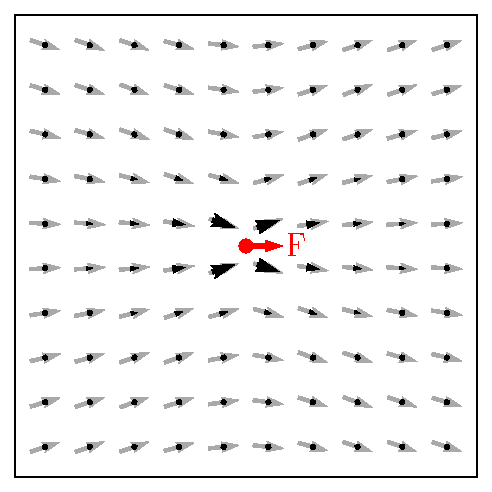
\includegraphics[width=0.49\columnwidth]{stokeslet1.pdf}
  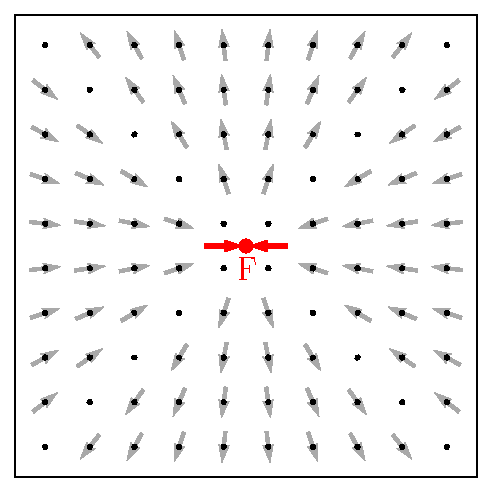
\includegraphics[width=0.49\columnwidth]{stresslet1.pdf}
  \caption{Flow fields due a Stokeslet (left) and a stresslet (right) centered at the origin (red dot). The black arrows display the velocities, while their directions are also indicated by the gray arrows. The flow fields are both axi- and fore-aft symmetric. Note the difference in the velocity magnitude of the two flows.}
  \label{fig:lets}
\end{figure}

Finally, for a sphere of radius $a$, translating with velocity $\bm U$ and rotating with angular velocity $\bm \Omega$, its total drag, torque, and stresslet are given by the \emph{Fax\'{e}n's laws},
\begin{subequations} \label{eq:faxen}
 \begin{equation}
   {\bm F}^{d} = 6\pi\mu a\bigg( (1+\frac{a^2}{6}\nabla^2){\bm u^\infty - {\bm U}} \bigg) ,
 \end{equation}
 \begin{equation}
  {\bm T}^{d} = 8\pi\mu a^3 ({\bm \omega}^\infty - {\bm \Omega}),
 \end{equation}
 \begin{equation}
   {\bm S} = \frac{20}{3}\pi\mu a^3 \bigg( 1+\frac{a^2}{10}\nabla^2 \bigg) {\bm E}^\infty ,
 \end{equation}
\end{subequations}
where $\small {\bm E}^\infty=(\nabla {\bm u}^\infty + (\nabla {\bm u}^\infty)^T)/2$ is the rate-of-strain tensor.


\section{Droplet interactions in shear flows}

The preceding section presents the most basic solutions of the Stokes equation in the presence of one particle.
In practice, however, it is rarely the case particles or droplets exist in isolation.
Particles tend to abound; and they often interact with each other through various types of hydrodynamic or non-hydrodynamic mechanisms, giving rise to a multitude of phenomena in natural or artificial conditions.
For example, soap bubbles are always in a cluster due to the interfacial capillary attraction, while the same underlying principle can be applied to manipulate droplet motions on a surface to aid liquid handling \citep{vapour-sensing}.
To offer at least some partial insights on the hydrodynamics, we highlight recent theoretical developments of droplet interactions in bulk microflows, starting from the simplest case of two particles immersed in unbounded simple shear flows.

\subsection{Pair interactions in unbounded flows}

Among the early studies of suspension hydrodynamics, \cite{batchelor_green_1972} solved completely the dynamics of two rigid spheres of arbitrary sizes subject to a background fluid motion whose velocity at infinity is a linear function of position, \ie
${\bm u}^\infty \sim {\bm E}^\infty \cdot {\bm x} + {\bm \omega}^\infty \times {\bm x}$ as $\abs{{\bm x}} \to \infty$.
The solution entails the relative velocity of the two sphere centers and their force dipole strengths (related to the effective viscosity of the suspension, see Section \ref{sec:sus-rheo}), and is given in terms of several geometric parameters functions of the spheres' relative position and size ratio.
In the special case of two equal-sized spheres suspended in simple shear flows, the relative velocity can be integrated numerically to yield a trajectory map as in Figure \ref{fig:BG-traj}.
Here, two types of trajectories can be identified:
(i) an \emph{open} trajectory where one particle approaches the other particle from one side, overtakes it, and continues in the same direction to infinity; and
(ii) a \emph{closed} trajectory where two particles stay bound and rotate around each other permanently regardless of how far they may separate temporarily.
It was noted by the authors that, under such ideal conditions (\eg smooth particle surface), the separatrix between open and closed trajectories encloses an infinite volume.
Furthermore, if the two particles are once aligned in the flow direction, they will form a closed loop forever.
% or we can call this a naive man's projection of his relationship ;)

\begin{figure}%[t]
  \centering
  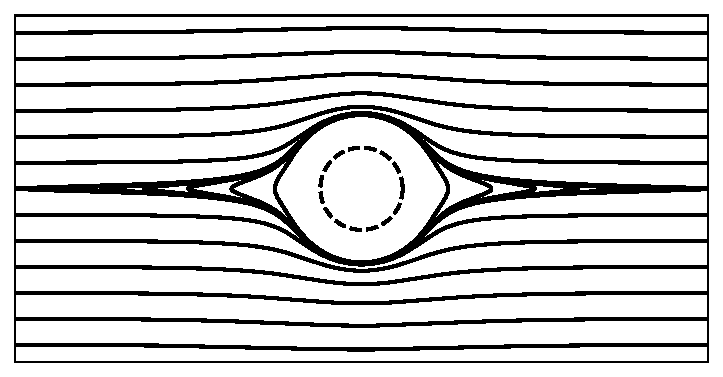
\includegraphics[width=0.8\columnwidth]{BG-traj4.pdf}
  \caption{Trajectory map of two equal spheres in unbounded simple shear flows. The dashed circle indicates the reference sphere, while the solid lines depict the relative trajectories of the second sphere in all planes of axisymmetry, which include the shear plane.}
  \label{fig:BG-traj}
\end{figure}

\cite{Zinchenko1983,Zinchenko1984} considered the problem when the two particles are ``fluid spheres''.
Specifically, he calculated the scalar parameters introduced in \cite{batchelor_green_1972} for two identical droplets, and showed that they are functions of the relative position and viscosity ratio, $\lambda$, defined as the ratio between the droplet and the solvent viscosities.
For $\lambda=$ 0.25 to 20, the phase diagram  in simple shear flows has similar topological features to the case of rigid particles,\footnote{Different types of trajectories were also hypothesized, which may only exist in the case of liquid drops. See \cite{Zinchenko1984} for details.} \ie an open region and a closed region, though its asymptotic limit depends on the viscosity ratio and short-range non-hydrodynamic interactions, cf.\ the DLVO theory.

For the above analysis to hold for liquid droplets, an additional constraint must be satisfied, \ie Ca $\ll 1$.
This is usually the case for microfluidic applications. For instance, recall the case considered in the beginning of Section \ref{sec:stokes-flows}, and suppose it is an oil droplet traveling in water under a relatively large local shear rate of $\dot{\gamma}=10^3$ s$^{-1}$. The surface tension coefficient would be around 0.05 N/m, depending on surfactants and the temperature, resulting in Ca $=\mu(a\dot{\gamma})/\gamma \sim 10^{-4}$. Clearly, the capillary number is small enough for the droplet to remain spherical in the flow.

We note that, in both cases, the relative particle velocity is proportional to the shear rate of the underlying flow. That is, doubling the shear will result in twice as fast relative motions between the particles, though the relative velocity remains much smaller than the absolute velocity in the lab frame (typically two orders-of-magnitude smaller). Hence, these are truly slow, but long-range, interactions.

When particles are at close contact, say the surface gap $h \ll a$, with $a$ being the particle radius. Then, the hydrodynamic interaction will be dominated by the lubrication term. Specifically, the lubrication force diverge as $a/h$ in the longitudinal direction, and as $\log(a/h)$ in the transverse directions \citep{jeffrey_onishi_1984, jeffrey1992}. Qualitatively, lubrication functions as a dashpot that prevents incoming particles from colliding and separating particles from overshooting. These will be further discussed and demonstrated in Section \ref{sec:num-dem} and \emph{Papers 7 \& 8}.


\subsection{Pair interactions under weak confinement}

When boundaries cannot be neglected in a binary encounter, how will the particle interactions be modified from the \cite{batchelor_green_1972} (BG) solution?
Before answering this question, observe that walls may be mathematically replaced with carefully chosen reflection images of the original particles such that the boundary conditions along the walls remain unchanged \citep{blake_1971, LironMochon}.
Therefore, we expect pair interactions in bounded flows to differ \emph{qualitatively} from the unbounded ones.

Beginning with the simplest case where only one wall is remotely present, \cite{Fouxon_Rubinstein2019} recently derived the relative velocity of two rigid particles as a sum of the BG's velocity and a wall-correction term (\emph{Paper 4}). The solution is constructed from an boundary integral representation of channel flows using multipole expansions similar to Eq.\ \eqref{eq:multipole}, see \cite{Fouxon_2017} (\emph{Paper 3}) for details.
Figure \ref{fig:itzhak-boris} illustrates the main results.
Here, the lines depicts the relative trajectories of the second particle in the shear plane, where the velocity is in the $x$ direction and increases with $z$. The wall is located at $z=-z_0$.
Remarkably, there exist two types of closed trajectories (in blue) and two types of open trajectories (in red).
Close to the origin, a degenerate of the BG-type closed trajectory is singly connected to an open trajectory at an unstable saddle point at distance $r_s$ from the origin.
The latter is not admissible in BG, as the particles swap their $z$ coordinates after a binary encounter rather than returning to the original positions.
Such open trajectories have been previously termed ``swapping trajectories'' and recognized as a wall-induced cross-streamline particle migration mechanism, attributing to the anomalously large self-diffusivity observed in a dilute suspension measurement \citep{Zarraga_Leighton2002, zurita-gotor_2007}.
Our derivation and numerical simulations independently verify this result.

\begin{figure}%[t]
  \centering
  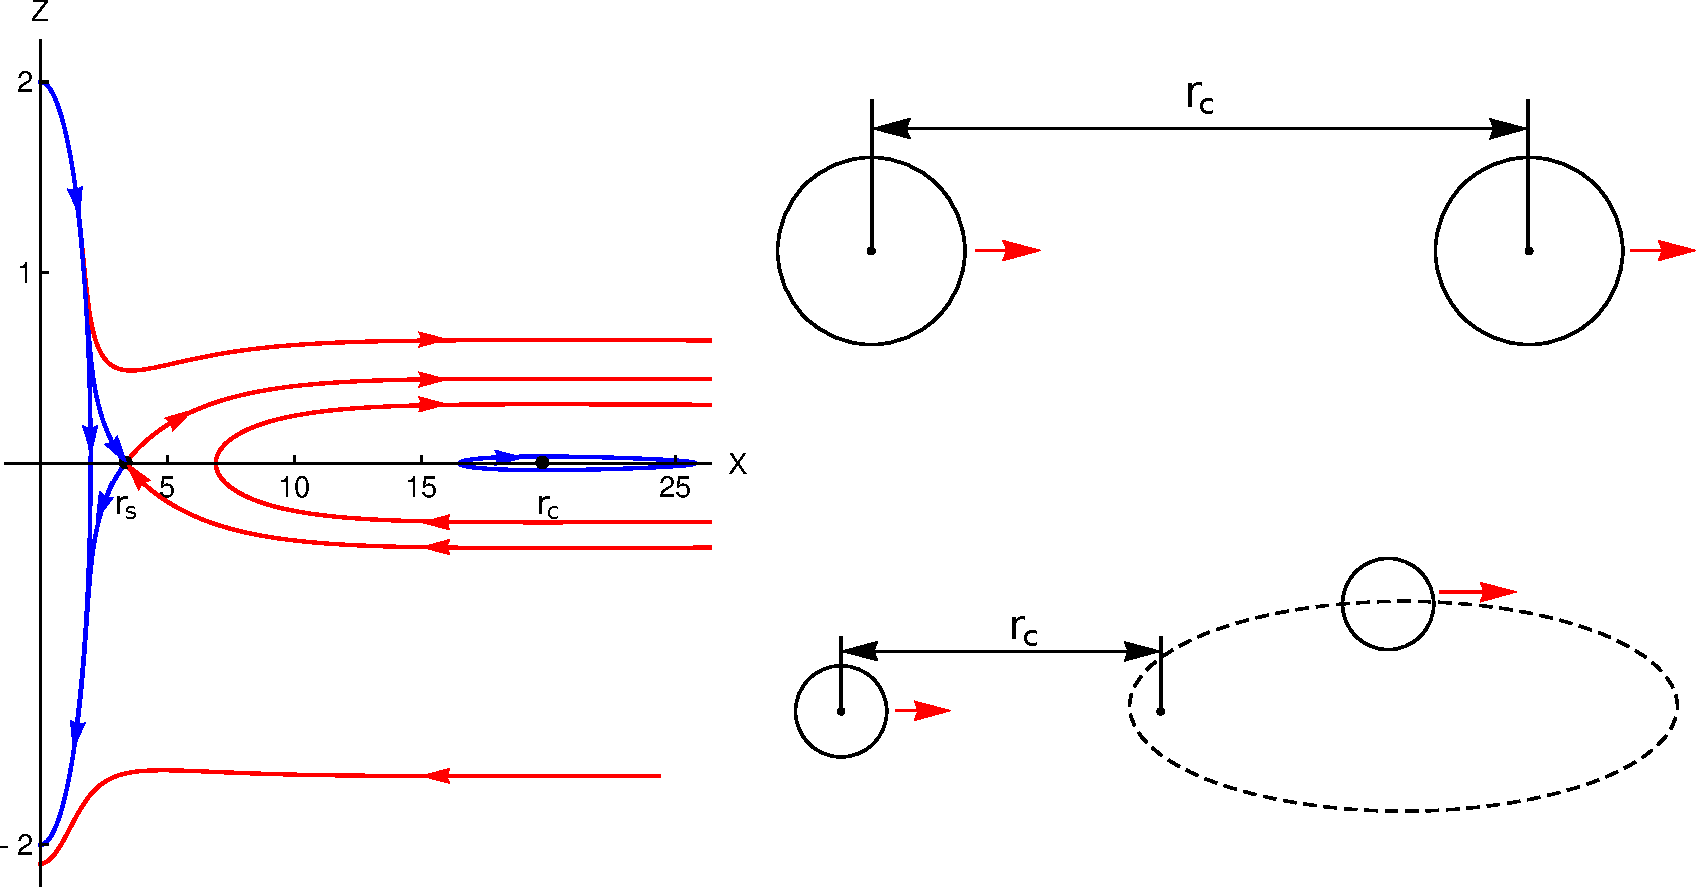
\includegraphics[width=\columnwidth]{itzhak-boris.pdf}
  \caption{
  (left) Trajectory map of two equal spheres in simple shear flows bounded by a distant wall. The distance between the reference particle (located at the origin) and the wall is $z_0=5$ (in units of particle radius, same for the labels of the plot). $r_s$ and $r_c$ denote the saddle point and the neutral equilibrium point, respectively.
  (right) Schematic illustrations of the stationary configuration (upper) and the dancing trajectory (lower).}
  \label{fig:itzhak-boris}
\end{figure}

Extending further away from the reference particle, we identify a new class of closed trajectories along which the second particle rotates around a neural equilibrium center. Note that, despite a distant wall, the trajectories remain axisymmetric with respect to the $x$ axis. Thus, all points on the circle $x^2+y^2=r_c^2$ are stationary configurations.
Slightly moving away from the center point, the second particles will revolve perpetually as it is convected by the flow; hence, we call them the ``dancing trajectories'' (see Figure \ref{fig:itzhak-boris}, right).
The positions of these critical points are approximately related to the wall separation alone. Specifically, $r_s=(32z_0^3/15)^{1/5}$ and $r_c \approx 4z_0$.
Overall, the wall is a singular perturbation to the free-space particle interaction.

\medskip
A few final remarks are in order before we proceed to more confined geometries.
%, it may be helpful to reflect on the physcial insights that can be gained from the theoretical analyses.
Firstly, in a dilute suspension of inertialess particles in Stokes flows, up to leading order in the particle-particle and particle-wall separations, the trajectory of one particle is the same as the fluid streamline resulting from the rest of the particle(s)/wall(s). Therefore, a comparison of the particle and fluid velocities has at least a qualitative meaning, or even quantitatively if the separations are large \citep{zurita-gotor_2007}.\footnote{This, of course, will be invalid if there are sufficient symmetry-breaking short-range interactions, see \eg \emph{Paper 2}.}
This can be more readily seen from the opposite statement, \ie if the particle trajectories are available, then the flow field can be qualitatively constructed using the particles as tracers.

\begin{figure}%[t]
  \centering
  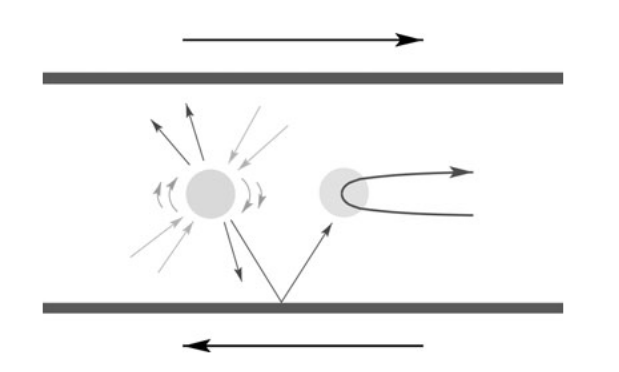
\includegraphics[width=0.55\columnwidth]{stresslet_reflection.png}
  \caption{Schematic of the wall reflection of the stresslet flow (cf.\ Figure \ref{fig:lets}) induced by one particle and its qualitative effect on the other particle. Reproduced with permission from \cite{zurita-gotor_2007}, \textcopyright \enspace Cambridge University Press.}
  \label{fig:stresslet-refl}
\end{figure}

Secondly, the effect of a rigid boundary on particle interactions can sometimes be intuitively predicted by image analyses utilizing basic solutions of the Stokes equation.
For example, \cite{zurita-gotor_2007} performed a relatively simple analysis to explain the flow reversal pattern (\ie the swapping trajectories) by calculating the scattering flow.
As sketched in Figure \ref{fig:stresslet-refl}, the wall reflection of the stresslet flow (since the particles are force-free) produces a vertical velocity component consistent with what is required for the position swapping (see \cite{zurita-gotor_2007} for the detailed calculations). This flow, despite being very small, is what causes the second particle to be shielded from the first one.

Thirdly, we note that these observed particle interactions may be superimposed pairwise to infer the collective dynamics of a group of particles in similar conditions.
To illustrate this point, we simulated two rigid particles in a periodic channel (thus mimicking a 1D crystal) and observed a crossover from permanent separation of the particle pair (for $0.32 \lessapprox z_0/H \lessapprox 0.68$) to a trapping state (for $z_0/H \lessapprox 0.32$ or $z_0/H \gtrapprox 0.68$), where $H$ is the channel height (same setup and notation otherwise, cf.\ Figures \ref{fig:itzhak-boris} and \ref{fig:stresslet-refl}).
Qualitatively, the former results from cross-stream migrations that resemble the BG open trajectories, while the latter is due to position swappings with neighbouring particles strongly influenced by the wall.
See \cite{Beatus2006, Janssen2012, Uspal2013} for a few more analogous and vivid demonstrations.

\begin{figure}%[t]
  \centering
  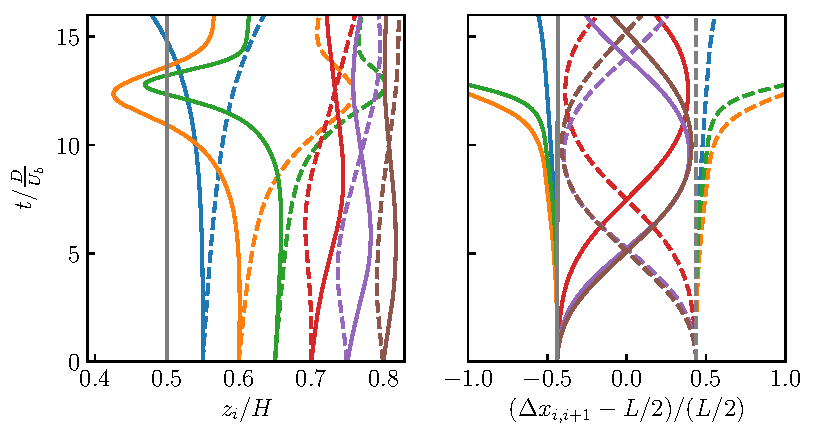
\includegraphics[width=0.9\columnwidth]{H3.pdf}
  \caption{Evolution of a particle chain under various initial vertical positions (indicated by the color). The periodic channel has a height of $H=6$ and a length of $L=8$, both in units of particle radius. The solid and dashed lines denote the up- and downstream particles in the two-particle system, respectively. For $0.32 \lessapprox z_0/H \lessapprox 0.68$ (only a half plane is shown due to symmetry), the lines diverge (see the right panel) indicating a permanent separation.}
  \label{fig:xover}
\end{figure}

%%neglect this since it's not theoretical
%We also show static pair under depletion force (\emph{Paper 2}).
%\begin{figure}%[t]
%  \centering
%  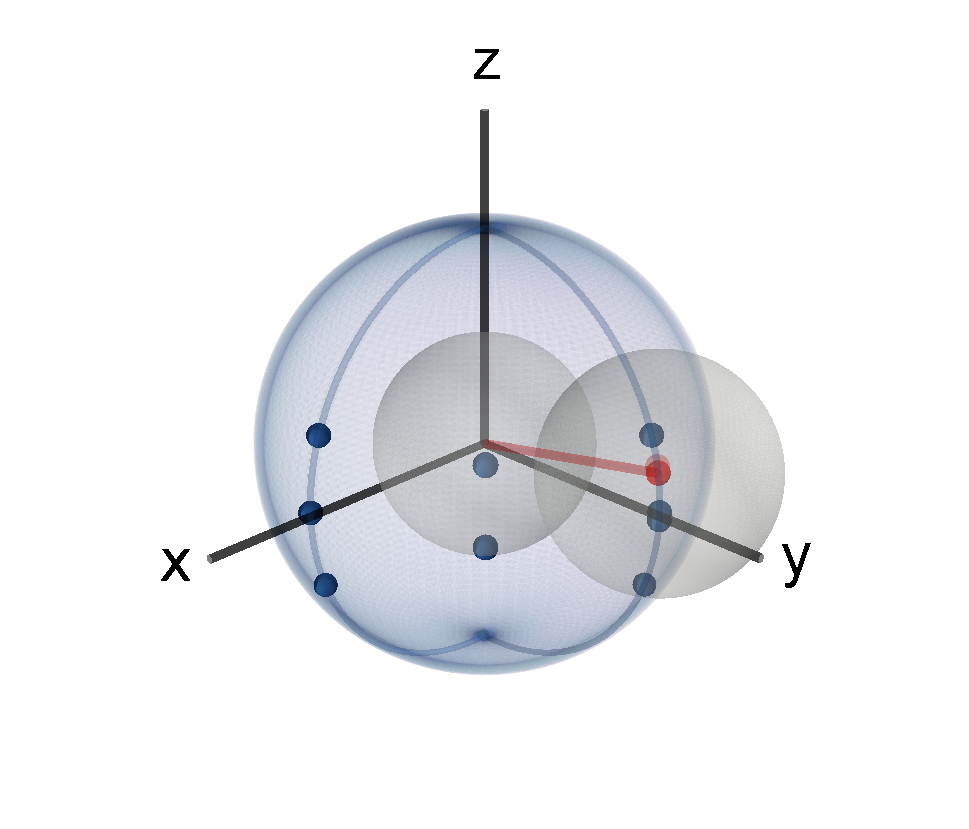
\includegraphics[width=0.32\columnwidth]{shell1.png}
%  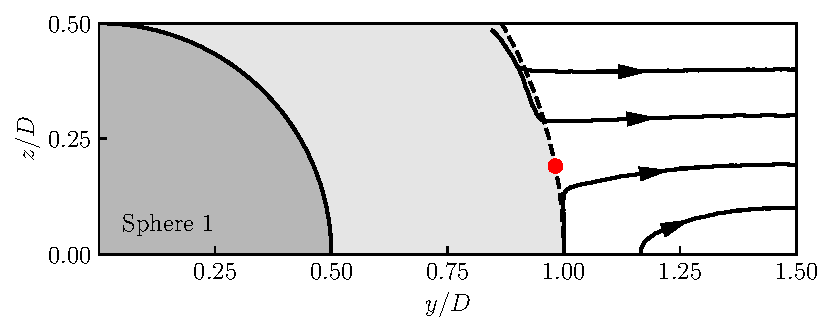
\includegraphics[width=0.65\columnwidth]{traj.pdf}
%  \caption{Trajectory map of two droplets in ...}
%  \label{fig:shear-align}
%\end{figure}


\subsection{Droplet interactions in quasi-two-dimensional geometries}
\label{subsec:drop-confined}

The last two decades has witnessed a boom of studies on hydrodynamic interactions in strongly confined geometries owing to the development of microfluidics \citep{Cui_etal_2002, Cui2004, tlusty, Davit_2008, q2d_Beatus}. At a first glance, increasing the confinement seems to complicate the problem as the boundary conditions becomes non-negligible (as opposed to being infinitely away), see \eg \cite{LironMochon, Fouxon_Rubinstein2019}. However, by returning to the physical origin of the equations, one can surprisingly gain a useful insight applicable to a wide range of geometries and particle sizes \citep{Diamant_2005}. Below, we exemplify two such conditions, one in which the interacting droplets are confined between two rigid planes, the other between free surfaces. The solutions are simplified by focusing on the far-field interactions and realizing that the problem is \emph{quasi-two-dimensional} (q2D). 

\medskip
Consider the flow between two parallel plates where the gap $H$ is much smaller than the other two dimensions (say $x$ and $y$); such geometry is commonly known as the \emph{Hele Shaw cell}. Then, from the lubrication theory, the velocity of the flow within the thin layer is approximately prescribed as 
 \begin{equation} \label{eq:hele-shaw}
  \begin{aligned}
    {\bm u}(x,y,z) \approx -\frac{z(H-z)}{2\mu} \nabla p(x,y),
  \end{aligned}
 \end{equation}
where the vertical components of the velocity and pressure are neglected, though ${\bm u}$ remains $z$-dependent. Hence, the flow is quasi-two-dimensional.

Under such conditions, the velocity field is irrotational and satisfies the boundary conditions of zero normal components at a rigid boundary in the horizontal plane \citep{Batchelor}. That is, a moving droplet (shaped as a pancake in q2D) shall have zero mass flux through its edge, not no-slip. With these requirements, it can be shown that the flow, created by the drop far from its surface, is proportional to
%Similar to the derivation for the Stokeslet, the flow ${\bm u}$ due to a moving droplet can be approxmiately derived, which has the following far-field structure
\begin{equation} \label{eq:dipolar}
 \begin{aligned}
   {\bm B}^s({\bm x}) \approx -\frac{\alpha H}{\mu} \bigg( \frac{{\bm I}}{\abs{\bm x}^2} -\frac{ 2{\bm x}{\bm x} }{ \abs{{\bm x}}^4} \bigg),
   \quad \textrm{for} \quad \abs{\bm x} \gg H,
 \end{aligned}
\end{equation}
where $\alpha$ is a dimensionless prefactor depending on the confinement \citep{Diamant}.

Physically, the above equation describes a 2D \emph{mass dipole} that displaces the surrounding fluid as the droplet moves.
Mathematically, it is the q2D Oseen tensor that approximates the velocity due to forcing on a moving droplet from afar, \ie ${\bm u} \sim {\bm B}{\bm F}$.
Specifically, ${\bm u}$ decays with the distance as $1/\abs{\bm x}^2$, which is faster than the free-space Stokeslet flow, but surprisingly slower than the flow caused by a moving particle near a single plate \citep{Cui2004}.
Heuristic arguments based on conservation laws have been proposed to explain these scaling differences, see \cite{Diamant} for details.

\begin{figure}%[t]
  \centering
  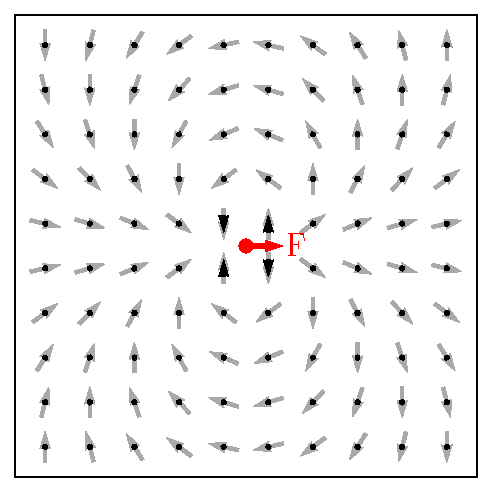
\includegraphics[width=0.49\columnwidth]{dipolar.pdf}
  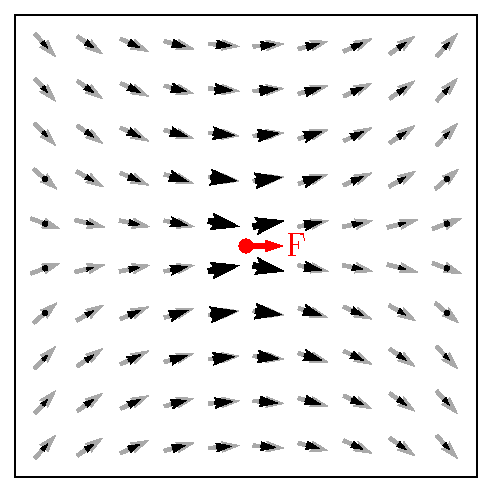
\includegraphics[width=0.49\columnwidth]{soap.pdf}
  \caption{Flow fields due a moving particle in a Hele-Shaw channel (left) and in a soap film (right). Both systems are quasi-two-dimensional.}
  \label{fig:q2d}
\end{figure}

To see the flow structure more clearly, we plot the dipolar flow resulting from a horizontal force in Figure \ref{fig:q2d} (left).
Here, the most salient feature is the negative transverse coupling of the droplet motion, \ie droplets exert ``antidrag'' on one another when moving perpendicular to their connecting line \citep{Cui2004}.
This pattern, however, can also be reversed if the droplets are driven by the flow. In that case, droplets lagging behind the undisturbed Hele Shaw flow will convey each to downstream directions to which they also travel \citep{Beatus2006}.
%Identification of this dipolar interaction mechanism has led to many microfluidic-based droplet manipulations, see \cite{q2d_Beatus} for a recent review.
%(iii) At large distances, the pair interaction is independent of concentration within the experimental accuracy. 
We note that the magnitude of typical dipolar flows are very small comparing to the driven flow in a dilute suspension. Even in the limit of $a/H \to 0$, where $a$ is the particle radius, the prefactor in Eq.\ \eqref{eq:dipolar} is analytically found to be $\alpha=3/(32\pi)\approx 0.030$ \citep{LironMochon}.
However, if the droplet nearly blocks the channel, the resulting flow will be plug-like and has a constant velocity \citep{q2d_Beatus}.

\medskip
An interesting variation of the aforementioned q2D system is to change the boundary from solid plates to free surfaces. Physically, this could be realized by trapping colloidal particles within a soap film using optical tweezers \citep{Leonardo_etal_2008}.

The Oseen tensor describing the long-range interactions within such a system is given as \citep{Leonardo_etal_2008, Diamant}
\begin{equation}
 \begin{aligned}
   {\bm B}^f({\bm x}) \approx \frac{1}{4\pi\mu H} \bigg[ \big( \ln(\nicefrac{1}{\kappa r}) -1 \big) {\bm I} +\frac{{\bm x}{\bm x} }{ \abs{{\bm x}}^2} \bigg],
   \quad \textrm{for} \quad \abs{\bm x} \gg H,
 \end{aligned}
\end{equation}
where $\kappa^{-1}$ is a cutoff length, \ie the radial velocity component vanishes for $\abs{\bm x} \geq \kappa^{-1}$, and it is necessitated by the lateral system size or finite liquid inertia.\footnote{By definition, $\kappa^{-1} \gg H$.}
Upon visualization of the resulting flow field (Figure \ref{fig:q2d}, right), it is obvious that particle interactions have a much longer range in free-standing liquid films. Furthermore, the transverse motions remain strongly coupled at distances where the longitudinal mode has mostly decayed.
The slow logarithmic decay comparing to the dipolar flow in a Hele Shaw cell is physically owing to the momentum conservation at the liquid boundaries, as opposed to momentum absorption by the rigid plates \citep{Diamant}.
This difference may have implications to protein transport in biological membranes \citep{Saffman3111}.

\medskip
Finally, we emphasize that the above analyses are strictly limited to far-field interactions as a consequence of the dimensionality reduction.
To consider near-field interactions, the full Navier-Stokes or Stokes equations often have to be solved to accurately resolve the detailed flow fields near the droplet, see \eg \cite{zhu_gallaire_2016, flow-assist}. 
In general, q2D analyses are applicable if the system contains a limiting length scale smaller than any other relevant distances, and if a long time evolution is of interest.
3D calculations, however inconvenient, cannot be avoided in most other situations.


\section{Bulk properties and suspension rheology}
\label{sec:sus-rheo}

When the number of particles is large within a suspension, analytical calculations of their relative motions can quickly become forbidden due to the complexities of the $N$-body problem.\footnote{Theoretically, $N = 3$ is the lower bound to break the time reversal symmetry.}
This is because, despite the fact that we know how to calculate the interaction at the individual level, the collective dynamics are often in regimes that are far from equilibrium, for which there is no established theoretical framework to rely on.
Even if we are primarily interested in averaged properties of a suspension, \emph{a priori} predictions can seldom be made as the \emph{microstructure}, \ie the spatial arrangement of each suspending particle, both determines and is determined by the bulk motion in a dynamic way \citep{Brady_Bossis1988}.
Nevertheless, in the following, we will introduce a few macroscopic properties of particle suspensions and show how they can be related to certain \emph{measurable} or \emph{computable} system parameters. The purpose is to provide a basic physical understanding and, in particular, the rheological characterizations of a particulate system.

\subsection{Sedimentation velocity}

For a sedimenting suspension, the average velocity is given by
\begin{equation}
 \begin{aligned}
   \langle {\bm U} \rangle = \langle {\bm M} \rangle \cdot {\bm F},
 \end{aligned}
\end{equation}
where ${\bm M}$ is the \emph{mobility tensor} that relates the overall forcing ${\bm F}$, such as gravity, to the particle velocity ${\bm U}$, cf.\ Eq.\ \eqref{eq:stokeslet}; and $\langle \cdot \rangle$ denotes an average over all particles followed by an average over all configurations. Instantaneously, ${\bm M}$ depends only on the particle configuration instead of the velocity \citep{durlofsky_brady_bossis_1987}; its diagonal blocks represent the single-body drag coefficients, while its off-diagonal blocks embody the hydrodynamic interactions between the particles. In addition, for rigid particles undergoing purely hydrodynamic interactions, ${\bm M}$ is symmetric and positive definite due to the dissipative nature of the system \citep{graham_2018}. This property facilitates the proper inversion of ${\bm M}$ to produce the many-body approximation to the resistance matrix as required in some reduced-order computational models, see Section \ref{sec:num-dem}.

\subsection{Diffusion tensor}

The $N$-particle diffusion tensor $\bm D$ can be generalized from the Einstein relation \citep{Einstein1905} and is given by
\begin{equation}
 \begin{aligned}
   {\bm D} = k_BT{\bm M},
 \end{aligned}
\end{equation}
where $k_B$ is the Boltzmann constant, $T$ is the temperature, and ${\bm M}$ is again the mobility tensor. That is, diffusion and mobility have the same qualitative meaning for a particulate system.

For non-Brownian suspensions, several particle diffusivities may be defined, though the motion of a particle is typically not diffusive except at short and long times \citep{Brady_Bossis1988}.
In the short-time limit, the self-diffusivity ${\bm D}_0^s$ can be taken as the diagonal of $\bm{D}$ per particle and average over all particles; whereas in the long-time limit, the self-diffusivity ${\bm D}_\infty^s$ is usually defined with the mean-square displacement, \viz
\begin{equation}
 \begin{aligned}
   {\bm D}_\infty^s = \lim_{t \to \infty} \frac{ \langle \big({\bm x}_i - {\bm x}_{i,0} )^2 \rangle_i }{2t},
 \end{aligned}
\end{equation}
where ${\bm x}_i$ is the position of particle $i$ at $t \to \infty$, ${\bm x}_{i,0}$ is its starting position, and $\langle \cdot \rangle_i$ is an average over $i$. Note that self-diffusivities are vectors of the same size of the dimensionality of the space, $d$. For an isotropic suspension, it can also be expressed as a scalar by averaging the components of ${\bm D}^s$ over $d$.

\subsection{Stress tensor}

One of the central tasks of rheology is to determine the bulk stress tensor $\langle \bm{\Sigma} \rangle_i$ of a flowing material, expressed as \citep{batchelor_1970, batchelor_1977}
\begin{equation} \label{eq:stress-tensor}
  \begin{aligned}
    \langle \bm{\Sigma} \rangle_i = -\bm{\Pi} +2\mu \bm{E}^\infty + \frac{N}{V} 
    \bigg(\langle \bm{S}^H \rangle_i + \langle \bm{S}^B \rangle_i +\langle \bm{S}^A \rangle_i \bigg), 
  \end{aligned}
\end{equation} 
where $V$ is the enclosing volume,
$N$ is the number of particles,
and $\bm{S}$'s denote the stresslets due to various particle interactions, including the hydrodynamic ($H$), Brownian ($B$), and any other applied ($A$) forces, as written.
Apart from the viscous stress tensor, $-\bm{\Pi} +2\mu \bm{E}^\infty$, due to the underlying flow, the rest of the terms in Eq.\ \eqref{eq:stress-tensor} are the particle contribution.
In general, these stress components are all related to the suspension microstructure.
In the case of the hydrodynamic stresslet, it can be computed as
\begin{equation} 
  \begin{aligned}
    \langle \bm{S}^H \rangle_i = - \langle \bm{R}_{SU}\cdot(\bm{U}-\bm{U}^\infty) - \bm{R}_{SE}:\bm{E}^\infty \rangle_i , 
  \end{aligned}
\end{equation}
where $\bm{R}_{SU}$ and $\bm{R}_{SE}$ are configuration-dependent resistance matrices that resemble $\bm{M}^{-1}$.
See Section \ref{subsec:sd} and \emph{Paper 7} for further details.

\bigskip
Suppose that the bulk stress tensor has been determined, then a number of \emph{effective} rheological properties can be readily extracted as follows.
Specifically, we focus on non-Brownian, rigid, neutrally buoyant spheres suspended in a Newtonian fluid with viscosity $\mu$ undergoing a simple shearing motion in the $xy$ plane with shear rate $\dot{\gamma}$.

\begin{enumerate}

\item Suspension viscosity $\eta_s=\bm{\Sigma}_{xy}/(\mu\dot{\gamma})$.

\medskip
When particles are added to a fluid, the increase of the suspension viscosity is linear with the shear rate if there is no other associated time scale in the system \citep{hinch_2011}.
Moreover, dimensional analysis indicates that there is only one independent variable, the volume fraction of the particles, $\phi$.
For very dilute suspensions (typically up to volume fraction $\phi \approx 0.05$), \cite{Einstein_1906, Einstein1911} has shown that $\eta_s = 1 + 2.5\phi$, assuming the particles only perturb the surrounding flow but do not interact with each other.
Including pair interactions, \cite{batchelor_green_1972b} calculated the suspension viscosity up to the quadratic order. For semi-dilute suspensions (up to $\phi \approx 0.15$) in simple shear flows, it follows $\eta_s = 1 + 2.5\phi + 5\phi^2$.
As the concentration continues increasing, analytical calculations of the stress tensor become difficult due to coupled hydrodynamic interactions and contact forces.
Plenty of empirical relationships have been proposed, such as that of \cite{Eilers1941}, $\eta_r=\mu[1+(5\phi/4)/(1-\phi/\phi_J)]^2$, where $\phi_J$ is the jamming fraction.
The latter may depend on the particle shape and friction coefficient.
For example, random close packing of frictionless sphere predicts $\phi_J \approx 0.64$, while in experiments suspensions usually jam under 60\% volume fraction.
See \cite{guazzelli_pouliquen_2018, Morris_annurev2020} for detailed reviews on the rheology of dense suspensions.
\bigskip

\item Particle pressure $\eta_n=-$Tr$(\bm{\Sigma})/(3\mu\dot{\gamma})$.

\medskip
Reminiscent of the osmotic pressure in a molecular fluid, particles in a suspension can generate an isotropic stress resulting from their hydrodynamic and other types of interactions \citep{brady--1993}.
Defined as the minus one-third the trace of the first moment of the surface stress acting on the particle, \cite{Jeffrey_morris_93} derived the analytical expressions for the cases of one and two particle(s) in linear flows. In the former case, a Fax\'{e}n law for the pressure moment is given as $S=4\pi a^3 p^\infty$, where $p^\infty$ is the ambient pressure due to the point force, cf.\ Eq.\ \eqref{eq:faxen}.
As the particle concentration increases, $\eta_n$ tends to diverge similarly to the suspension viscosity.
In simple shear flows, a possible constitutive relationship is suggested as $\eta_n=[\phi/(\phi_J-\phi)]^2$ \citep{Boyer_Guaz_Poul_2011}.
\bigskip

\item Normal stress differences $N_1=\bm{\Sigma}_{xx}-\bm{\Sigma}_{yy}$ and $N_2=\bm{\Sigma}_{yy}-\bm{\Sigma}_{zz}$.

\medskip
When the suspension is non-dilute, normal stresses can deviate from each other as a result of the anisotropic microstructure or particle collision.
This leads to the definitions of the first and second normal stress differences as above, where $x$, $y$, $z$ denote the flow, velocity-gradient, and negative vorticity directions, respectively.
$N_1$ and $N_2$ are usually normalized by the modulus of the shear stress, $\abs{\bm{\Sigma}_{xy}}$, since they also diverge as $\phi \to \phi_J$.
The exact relationship between $N_1$ or $N_2$ and $\phi$ have not been clearly found. The overall picture is that $N_1$ is mostly of hydrodynamic origin, while $N_2$ is large and negative due to particle collisions, which happen more frequently in the $xy$ plane \citep{guazzelli_pouliquen_2018}.
See \cite{seto_giusteri_2018} for further discussions.

\end{enumerate}



%===============================================================================
\chapter{Numerical Methods}
%===============================================================================


The previous chapter depicts the physical pictures of droplet interactions and suspension flow in a few simplified conditions.
In the current chapter, we peek in the technical details of various numerical methods when theoretical analyses are insufficient and the full equations have to be simulated to describe the coupled fluid and particle dynamics.
First, we discuss standard Navier-Stokes solvers along with different interface-tracking/capturing methods. Simulations adopting these approaches intend to resolve all spatial and temporal scales within the system, and sometimes qualify as \emph{direct numerical simulations} (DNS).
Then, we discuss a special class of methods that solves the particle dynamics without directly computing the flow, thus is much faster, but becomes invalid beyond the Stokes flow approximation. Depending on the level of simplifications, these may fall under the category of \emph{coarse-grained} dynamics.
In view of the large amount of numerical methods and the constant development of computational fluid dynamics (CFD) in the last several decades, the list of methods is by no means complete. For more comprehensive surveys of available numerical techniques for multiphase flow problems, see \cite{prosperetti_tryggvason_2007, Rosti2019}.


%-------------------------------------------------------------------------------

\section{Interface-resolved one-fluid methods}
\label{sec:fluid-methods}

The incompressible Navier-Stokes equations, Eqs.\ \eqref{eq:Navier-Sotkes}, can be solved numerically using the classical \emph{projection method} \citep{Chorin_1968} by repeatedly executing the following steps,
\begin{subequations} \label{eq:projection-method}
 \begin{equation} \label{eq:ab2}
  \begin{aligned}
   {\bm u}^* ={\bm u}^{(n)} +\Delta t \bigg(\frac{3}{2} {\bf RU}^{(n)}-\frac{1}{2} {\bf RU}^{(n-1)} \bigg),
  \end{aligned}
 \end{equation}
 \begin{equation} \label{eq:poisson}
  \nabla^2 p^{(n+1)} = \frac{\nabla \cdot {\bm u}^*}{\Delta t},
 \end{equation}
 \begin{equation} 
   {\bm u}^{(n+1)} = {\bm u}^* -\Delta t \nabla p^{(n+1)},
 \end{equation}
\end{subequations}
where
\begin{equation}
  {\bf RU}^{(n)} = -{\bm u}^{(n)} \cdot \nabla {\bm u}^{(n)} +\nabla^2 {\bm u}^{(n)} +{\bm f}^{(n)}.
\end{equation}
In the above, superscripts $^{(n)}$, $^*$, and $^{(n+1)}$ denote the discrete time-levels in step of $\Delta t$;
and $\rho$ and $\mu$ are assumed to be 1 for simplicity.
The flow field, $\bm u$, is updated in time via a fractional-step procedure, where the first sub-step, Eq.\ \eqref{eq:ab2}, utilizes the second-order Adams-Bashforth (AB2) scheme. Other temporal integration schemes, \eg the Runge-Kutta (RK) or Crank-Nicolson (CN) methods, can also be used or mixed-and-used depending on the numerical stability and desired accuracy.
In moderate-Reynolds-number systems, AB2 is typically favored over other schemes as it is easy to implement (comparing to implicit schemes such as CN) and relatively fast (comparing to high-order schemes such as third-order RK).

In order to evaluate the spatial derivatives in Eqs.\ \eqref{eq:projection-method}, the flow domain should be discretized so that either finite difference or weighted residual methods can be applied.
In essence, finite difference methods express the derivative as a truncated Taylor series expansion, while weighted residual methods assume that the solution can be represented analytically and they are usually formulated as one of the following better-known variants, including finite volume, finite element, or spectral methods \citep{Fletcher}.
Loosely speaking, finite difference and finite volume schemes are easier to implement on a structured grid; finite element methods are more flexible on non-Cartesian grids; and spectral methods have the highest order-of-accuracy.

Depending on the numerical condition and specific implementation, solving Eqs.\ \eqref{eq:projection-method} can be costly. The most computationally intensive part in a projection method is usually Eq.\ \eqref{eq:poisson}, where a Poisson equation for pressure must be solved numerically at each time step. Consequently, much work has gone into developing fast or iterative Poisson solvers that take advantage of fast Fourier transforms, Gauss elimination, or multigrid methods, see \cite{Buzbee_Golub_Nielson, Swarztrauber1977, multigrid_Brandt, Wesseling} for some early examples.

The above entails the most basic algorithm for single-phase flow.
When particles or droplets are present, the flow is \emph{multiphase} and additional equations may have to be introduced to describe the dispersed phase that modifies the underlying flow.
Below, we give a brief overview of some interface-tracking/capturing methods that have been developed along this direction.
The common feature of these methods is that they follow the the motion of finite-size particles without deforming the original grid where the fluid variables are defined on.
Hence, they can all be referred to as ``\emph{one-fluid}'' methods.


\subsection{Front-tracking methods}

Using discrete marker points to specify and track particle motions, front-tracking type-of methods are perhaps the most intuitive approach for modelling finite-size particles and have been used in multiphase flow simulations since the inception of super computers \citep{Daly1969, Viecelli_1969, Peskin, Glimm_1982, unverdi_tryggvason_1992a, tryggvason_bunner_esmaeeli_juric_al-rawahi_tauber_han_nas_jan_2001a, Pozrikidis_JCP2001, Muradoglu_Tryggvason_2014}.
The general methodology is to
(i) prescribe the particle location by distributing a set of Lagrangian points on the particle surface (see Figure \ref{fig:front-track}),
(ii) advect them using the local flow velocity, and
(iii) update the fluid properties and compute the extra forces at the updated particle position.
In the case of liquid droplets, (ii) and (iii) can be written as
\begin{equation} \label{eq:lagrangian}
 \begin{aligned}
   \frac{d \bm{X}_l}{dt} = \bm{u}(\bm{X}_l),
 \end{aligned}
\end{equation}
\begin{equation} \label{eq:surf-tension}
 \begin{aligned}
   \bm{f} = \gamma \kappa \bm{n} \delta (\bm{X}_l) ,
 \end{aligned}
\end{equation}
where $\bm{X}_l$, $l=1,2,\dots,N_L$ denote the positions of the Lagrangian points, $\bm u$ the local flow velocity, $\bm f$ the forcing term, $\gamma$ the surface tension coefficient, $\kappa$ the interface curvature, $\bm n$ the interface normal vector, and $\delta$ the Dirac delta function. Eq.\ \eqref{eq:surf-tension} corresponds to the normal stress jump condition due to surface tension, cf.\ Eq.\ \eqref{eq:stress-bc}. No-slip boundary conditions on solid particles can be represented in similar ways.

Despite the conceptual simplicity, there are several technical details that require careful treatment when implementing front-tracking methods.
First, due to deformation of the particle or non-uniformity of the flow field, the Lagrangian points may need to be redistributed, added, or deleted from time to time to ensure numerical stability and accuracy.
This is particularly cumbersome when events of coalescence or breakup occur.
Second, advection of the marker points requires interpolation of the velocity field, as the moving grid is generally non-aligned with the background fixed mesh.
Third, the internal boundary conditions (no-slip or surface tension) are to be constraint on the Eulerian mesh, thus a ``spreading'' procedure is necessary to feed the particle dynamics back to the flow. This is usually done with a smeared delta function.

With these in mind, now we describe a specific class of front-tracking methods.

\begin{figure}%[t]
  \centering
  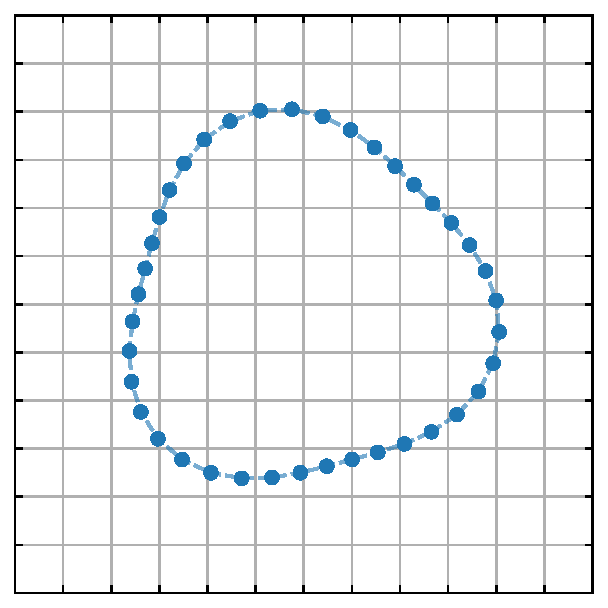
\includegraphics[width=0.6\columnwidth]{marker-points.pdf}
  \caption{Marker points on a triangular droplet.}
  \label{fig:front-track}
\end{figure}


\begin{algorithm}[h!]
 \ccc{\footnotesize //time marching} \\
 \For{$n=0,1,\dots,N$}{
  ${\bm u}_{ijk}^0 = {\bm u}_{ijk}^{(n)}$,
  ${\bf RU}_{ijk}^0 = {\bf RU}_{ijk}^{(n)}$, ${\bf RU}_{ijk}^{-1} = {\bf RU}_{ijk}^{0}$ \ccc{\footnotesize //fluid variables} \\
  $\bm{X}_l^{0}=\bm{X}_l^{(n)}$, $\bm{U}_p^{0}=\bm{U}_p^{(n)}$, $\bm{\Omega}_p^{0}=\bm{\Omega}_p^{(n)}$ \ccc{\footnotesize //particle motions} \\
  $\bm{F}_p^{0}=\bm{F}_p^{(n)}$, $\bm{T}_p^{0}=\bm{T}_p^{(n)}$ \\
  
  \ccc{\footnotesize //the RK3 loop} \\
  \For{$q=1,2,3$}{ 
   ${\bm u}_{ijk}^* = {\bm u}_{ijk}^{q-1} + \Delta t \big(-(\alpha_q+\beta_q)\nabla P_{ijk}^{q-3/2}+\alpha_q{\bf RU}_{ijk}^{q-1}+\beta_q{\bf RU}_{ijk}^{q-2} \big)$ \\
   ${\bm u}_{ijk}^{**,-1} = {\bm u}_{ijk}^*$ \\
   
   \ccc{\footnotesize //the mutli-direct forcing loop} \\
   \For{$s=0,1,\dots,N_s$}{
   
    \ccc{\footnotesize //the Lagrangian particle loop} \\
    \For{$l=1,2,\dots,N_l$}{
    $\bm{U}_{l}^{**,s-1} = \sum_{ijk} {\bm u}_{ijk}^{**,s-1} \delta_p( \bm{x}_{ijk}-\bm{X}_{l}^{q-1}) \Delta x \Delta y \Delta z$ \\
    $\bm{F}_{l}^{q-1/2,s} = \bm{F}_{l}^{q-1/2,s-1} + \frac{\bm{U}_{p}^{q-1}-\bm{U}_{l}^{**,s-1}}{\Delta t} $ \\
    }
    
    $\bm{f}_{ijk}^{q-1/2,s} = \sum_{l} \bm{F}_{l}^{q-1/2,s} \delta_p( \bm{x}_{ijk}-\bm{X}_{l}^{q-1}) \Delta V_l $ \ccc{\footnotesize //spreading} \\
    $\bm{u}_{ijk}^{**,s} = {\bm u}_{ijk}^* + \Delta t \bm{f}_{ijk}^{q-1/2,s} $ \\
   }
  $\nabla^2 \tilde{P} = \frac{1}{(\alpha_q+\beta_q) \Delta t} \nabla \cdot {\bm u}^{**,N_s}$ \ccc{\footnotesize //projection} \\
  ${\bm u}^{q} = {\bm u}^{**,N_s} -(\alpha_q+\beta_q)\Delta t \nabla \tilde{P}$ \ccc{\footnotesize //correction} \\
  $P^{q-1/2} = P^{q-3/2} + \tilde{P}$ \\

  \ccc{\footnotesize //integration of Newton-Euler} \\
  Evaluate $\bm{F}_{p}^{q}$ and $\bm{T}_{p}^{q}$ from the current particle configuration \\
  ${\bm U}_p^{q} = {\bm U}_p^{q-1} -\frac{\Delta t}{V_p}\sum_l  \bm{F}_{l}^{q-1/2,N_s} \Delta V_l +\frac{(\alpha_q+\beta_q) \Delta t}{2V_p}(\bm{F}_{p}^{q}+\bm{F}_{p}^{q-1})+\dots$ \\
  $\bm{X}^{q}=\bm{X}^{q-1}+\frac{(\alpha_q+\beta_q) \Delta t}{2}(\bm{U}_{p}^{q}+\bm{U}_{p}^{q-1})$ \\
  ${\bm \Omega}_p^{q} = {\bm \Omega}_p^{q-1} -\frac{\Delta t}{I_p}\sum_l \bm{r}_l^{q-1} \times \bm{F}_{l}^{q-1/2,N_s} \Delta V_l +\frac{(\alpha_q+\beta_q) \Delta t}{2I_p}(\bm{T}_{p}^{q}+\bm{T}_{p}^{q-1})+\dots$ \\
  }
  
  ${\bm u}_{ijk}^{(n+1)}={\bm u}_{ijk}^3$, ${\bf RU}_{ijk}^{(n+1)}={\bf RU}_{ijk}^3$  \\
  $\bm{X}_l^{(n+1)}=\bm{X}_l^{3}$, $\bm{U}_p^{(n+1)}=\bm{U}_p^{3}$, $\bm{\Omega}_p^{(n+1)}=\bm{\Omega}_p^{3}$ \\
  $\bm{F}_p^{(n+1)}=\bm{F}_p^{3}$, $\bm{T}_p^{(n+1)}=\bm{T}_p^{3}$ \\
 }
 \caption{A multi-direct forcing immersed boundary method for the coupled Navier-Stokes/Newton-Euler equations.}
 \label{al:ibm}
\end{algorithm}


\medskip
\paragraph{\bf Immersed boundary methods}

Pioneered by \cite{Peskin}, immersed boundary (IB) methods were originally used for modelling cardiac mechanics and associated blood flow, and have ever since been continuously modified and refined for multiphase flow simulations involving moving boundaries \citep{fadlun_verzicco_orlandi_mohd-yusof_2000a, Uhlmann, mittal_iaccarino_2005a, pinelli_naqavi_piomelli_favier_2010a, Wim-Paul_JCP_2012, favier_revell_pinelli_2014a}.
Here, the governing equations for the particle motion are the Newton-Euler equations,
\begin{subequations} \label{eq:newton-euler}
  \begin{equation} 
    \begin{aligned} \label{eq:force-balance}
      m_p \frac{d{\bm U}_p}{dt} = \int_{s} \bm{\sigma \cdot n} dA + {\bm F}_p, 
    \end{aligned}
  \end{equation}
  \begin{equation} 
    \begin{aligned}
      {\bm I}_p \frac{d{\bm \Omega}_p}{dt} + {\bm \Omega}_p\times({\bm I}_p{\bm \Omega}_p) =
      \int_{s} \bm{r} \times (\bm{\sigma \cdot n}) dA + {\bm T}_p,
    \end{aligned}
  \end{equation}
\end{subequations}
where ${\bm U}_p$ and ${\bm \Omega}_p$ denote the translational and angular velocities of particle $p$;
$m_p$ and ${\bm I}_p$ are its mass and moment-of-inertia tensor in the body frame (scalar for spheres); and 
${\bm F}_p$ and ${\bm T}_p$ stand for the total force and torque (except for the viscous stress contributions, which are represented by the integral terms) exerted on the particle center-of-mass.

The feedback of the particle on the fluid flow are embedded in a diffuse body-forcing term, $\bm f$.
Depending on whether it is incorporated into the continuous equations before or after discretisation, IB methods can be broadly divided into \emph{continuous forcing} and \emph{direct forcing}.
Regardless of the approach, the spreading of the Lagrangian force onto the Eulerian mesh is realized with regularized Dirac delta functions, which may take different forms as long as $\sum_{ijk} \delta_p( \bm{x}_{ijk}-\bm{X}_{l}) \Delta x \Delta y \Delta z=1$ is satisfied for all $\bm{X}_{l}$.

To illustrate the overall algorithm, a pseudo code corresponding to the direct forcing IB method used in \emph{Paper 3} and \emph{Paper 4} for spherical particles is provided in Algorithm \ref{al:ibm}.
Here, the code is structured in three nested loops:
an outer time-marching loop to advance the unsteady solution,
an intermediate third-order Runge-Kutta (RK3) loop to integrate the fluid velocity along with the particle motion,
and an inner loop for multi-direct forcing iterations.
The notation is similar to previous formulations, cf.\ Eqs. \eqref{eq:projection-method} and \eqref{eq:lagrangian}, with minor omissions of terms or exceptions, such as the definition of ${\bf RU}$ (in Algorithm \ref{al:ibm}, it does not include $\bm f$).
The objective is to give an overall picture of the complexity of the code. For full details, see \cite{ Wim-Paul_JCP_2012}.


\subsection{Front-capturing methods}

Instead of meshing and tracking the moving boundary on a separate grid, an alternative approach is to capture the particle motion on the same grid at the expanse of an additional function. Such function may correspond to the local volume fraction of a dispersed phase, or measure a geometric quantity of the interface away from the particle.
Conceptually, it specifies the multiphase flow in a full Eulerian manner, and is sometimes referred to as \emph{Eulerian-Eulerian} methods (front-tracking methods would be called \emph{Eulerian-Lagrangian} methods).
Many numerical methods fall under the Eulerian-Eulerian framework. In the following, we will describe three of them (see Figure \ref{fig:front-capture}).
As an outline, a brief historical background will be given first, followed by the definition of the ``front-capturing'' function and its governing equation. We will also highlight the major advantages and disadvantages of each method on a general basis.
Finally, when coupling these front-capturing methods with a flow solver, the internal boundary conditions need to be imposed near the interface and, in principle, can be treated in exactly the same way as in front-tracking methods, cf.\ Eq.\ \eqref{eq:surf-tension}. We skip these details and refer the reader to \cite{Brackbill_JCP_1992, Fedkiw_JCP_1999, Lalanne_JCP_2015, Popinet_ARFM_2018, Gibou_Fedkiv_Osher, ICLS} for further discussions.

\begin{figure}%[t]
  \centering
  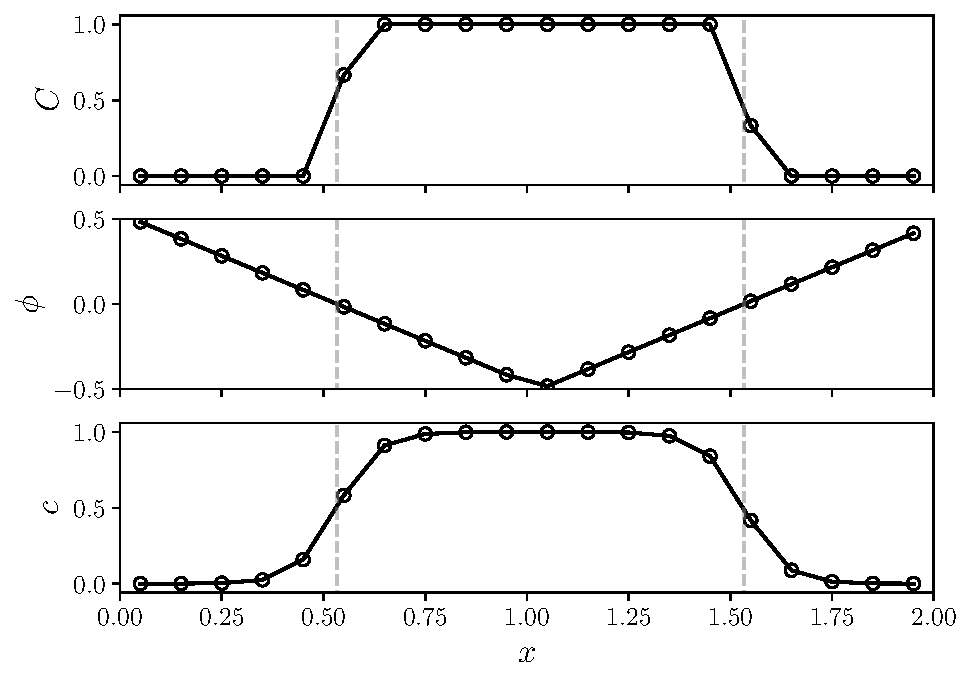
\includegraphics[width=\columnwidth]{front-capture-comp.pdf}
  \caption{Comparison of the three front-capturing methods for a 1D droplet of radius 0.5, centered at $x=1.033$. Markers indicate the nodal values of the representative functions. Dashed lines depict the boundary of the droplet.
  (upper) The volume-of-fluid representation, where $C=1$ inside the droplet.
  (middle) The level set representation, where $\phi >0$ outside the droplet.
  (lower) The phase field representation, where the profile is given by $c=0.5[1-\mathrm{tanh}(\phi/\epsilon)]$, with $\epsilon=0.1$.}
  \label{fig:front-capture}
\end{figure}


\medskip
\paragraph{\bf Volume-of-fluid methods}

First proposed in the 1970s, volume-of-fluid (VOF) methods were among the oldest interface-capturing methods for modelling free-surface flow \citep{Debar1974, hirt_nichols_1975, hirt_nichols_1981a}, and they remain as being the more popular methods for multiphase flow simulations within the CFD community \citep{Scardovelli_Zaleski_1999, gerris, pilliod_puckett_2004, xiao_honma_kono_2005a, mthinc2012, paris2019}.
The principle idea is, first, introducing a cell-averaged volume fraction, $C_{k}$, defined as
\begin{equation}
 \begin{aligned}
   C_{k} = \frac{1}{\Delta V_k} \int_{\Omega_k} H(\bm{x}) dV,
 \end{aligned}
\end{equation}
where $\Delta V_k$ is the volume of computational cell $k$, and $H(\bm{x})$ is a phase indicator function, given as
\begin{equation}
    H(\bm{x}_k)=
    \begin{cases}
        1 \quad \quad & \textrm{if $\bm{x}$ is in the reference fluid,} \\
        0 \quad & \textrm{otherwise}, \\
    \end{cases}
\end{equation}
then, obtaining the temporal variation of the local volume fraction by solving the following equation,
\begin{equation} \label{eq:vof-advect}
 \begin{aligned}
   \frac{\partial C_{k}}{\partial t} + \int_{\partial \Omega_k} (\bm{u \cdot n}_k) H(\bm{x}) dS =0,
 \end{aligned}
\end{equation}
where $\bm{n}_k$ denote the six normal vectors (in a 3D Cartesian mesh) of surfaces $\partial \Omega_k$, and $\bm u$ is the local divergence-free velocity.

Note that, in the above formulations, the \emph{total} volume of each fluid phase is conserved by construction.
For many engineering calculations, this is the minimum requirement for a long-time simulation to be meaningful and makes VOF appealing in a wide range of industrial problems, such as predicting the impact of ocean waves splashing on the ship hull or designing spray nozzles to enhance fuel mixing in engines.
On the other hand, to correctly capture the local interface motion, the volume flux in Eq.\ \eqref{eq:vof-advect} must be calculated accurately, which requires certain information of the local interface \emph{geometry}, such as the normal direction and curvature.
This further requirement is not straightforward knowing only the cell-averaged volume fraction (see Figure \ref{fig:front-capture} for a very simplified illustration), therefore, many efforts have been devoted to developing methods that either reconstruct the interface in an extra step (these methods are called geometric VOF) or represent the interface in certain ways such that the volume flux can be computed directly (these methods are called algebraic VOF). See \cite{mirjalili_jain_dodd_2017a} for a recent overview of the different methods.


\medskip
\paragraph{\bf Level set methods}

Another way to model interface evolution is to use level set (LS) methods \citep{sethian_1999a}.
Originally devised by \cite{Osher_Sethian_levelset}, LS methods encompass a broad class of algorithms and numerical schemes for ``front propagation'' with curvature-dependent speeds.
The mathematical machinery is rooted in the boundary-value and initial-value partial-differential-equations (PDE) perspective on moving interfaces.\footnote{It may seem similar to VOF methods in the sense that the both methods are Eulerian and the governing equations can be written in a similar way. However, the level set method embeds the \emph{geometry} of an interface, while VOF has the \emph{volume} embedding. This, together with that level set is Lipschitz-continuous and VOF is discontinuous, makes the two approaches fundamentally different. See Figure \ref{fig:front-capture}.}
Its applications include geometry, computer vision, fluid mechanics, combustion, tissue growth, path optimization, \etc
In terms of fluid mechanics, specifically, the last three decades has witnessed continuous numerical development in applying level set methods to multiphase flows, see \eg \cite{Mulder_JCP_1992, Sussman_JCP_1994, Sussman_JCP_2000, Enright_JCP_2002, Olsson_JCP_2005, Marchandise_JCP_2007, Desjardins_JCP_2008, Desjardins_JCP_2009, Aanjaneya_JCP_2013, Luo_JCP_2015, ICLS}. See also \cite{Gibou_Fedkiv_Osher} for a recent review.

The level set function, $\phi$, is classically defined as the signed distance to the interface $\Gamma$,
\begin{equation} \label{eq:ls-def}
    \phi({\bm x},t) = sgn({\bm x}) |{\bm x}-{\bm x}_\Gamma|,
\end{equation}
where $sgn({\bm x})$ is a sign function equal to $1$ or $-1$ depending on which side of the interface the observation point $\bm x$ lies, and ${\bm x}_\Gamma$ denotes the point on $\Gamma$ that has the shortest distance to $\bm x$.
That is, the interface can be parameterized by $\phi$ as $\Gamma = \{ {\bm x} ~ \rvert ~ \phi({\bm x},t) = 0 \}$.
The interface position is then advected according to the following level set equation,
\begin{equation} \label{eq:ls-eq}
  \frac{\partial \phi}{\partial t} + F \abs{\nabla \phi} = 0,
\end{equation}
where $F$ is a speed function.
From a PDE perspective, the above equation asserts that the entire level set evolution can be obtained by integrating $\phi({\bm x},t=0)$ forward in time.
In other words, Eq.\ \eqref{eq:ls-eq} is an initial value problem without boundary conditions.

Geometrically, the normal and the curvature of the interface can be readily derived from the level set as below,\footnote{Some authors express the curvature as $\kappa = -\nabla \cdot {\bm n}$, cf.\ \cite{Desjardins_JCP_2008, ICLS}. This is merely due to different sign conventions for the level set.}
\begin{subequations} \label{eq:ls-geo}
 \begin{equation}
    {\bm n} = \frac{\nabla \phi}{\abs{ \nabla \phi }},
 \end{equation}
 \begin{equation} \label{eq:curv}
    \kappa = \nabla \cdot {\bm n}.
 \end{equation}
\end{subequations}

When solving the level set equation for multiphase flow, the most natural choice for $F$ is the local flow velocity projected in the normal direction, \ie $F=\bm{u \cdot n}$, reducing Eq.\ \eqref{eq:ls-eq} to
\begin{equation} \label{eq:ls-avd}
  \frac{\partial \phi}{\partial t} + \bm{u} \cdot \nabla \phi = 0.
\end{equation}
However, any non-uniform flow will distort the LS field, making Eq.\ \eqref{eq:ls-def} invalid after a few advection steps and making the numerical solution unstable.
To remedy this problem, it is customary to perform an infrequent level set ``reinitialization'' to reshape $\phi$ into a distance function while preserving the interface location \citep{Sussman_JCP_1994}.
Various techniques have been developed to do so by \eg using fast marching methods \citep{sethian_1999a}, or solving a time-dependent Hamilton-Jacobi equation \citep{Sussman_JSC_1997, Russo_JCP_2000}. It is also possible to avoid this additional step by modifying $F$ such that the gradient of $\phi$ is always fixed, see \eg \cite{Adalsteinsson_JCP_1999}.

At this point, it is important to mention a critical numerical issue of classical level set methods. The problem is, even if Eq.\ \eqref{eq:ls-avd} is solved on an incompressible velocity field, there is no guarantee that the numerical solution will conserve the total enclosed volume; in practice, there is often significant ``mass loss''.
The reason for this problem is a combination of numerical dissipation, under-resolution, and lack of \emph{built-in} mass conservation properties in the numerical scheme.
Plenty of methods have thus been proposed to overcome such issues by using higher-order numerical schemes, coupling the LS with VOF or lagrangian particles, imposing additional mass constraints, \etc See \cite{ICLS} (\emph{Paper 1}) for a brief overview.

\begin{algorithm}[t]
 \ccc{\footnotesize //time marching} \\
 \For{$n=1,2,\dots,N$}{
  
  \ccc{\footnotesize //level set advection} \\
  $\phi^1 = \phi^{(n)} + \Delta t \cdot {AD}(\phi^{(n)})$ \\
  $\phi^2 = \frac{3}{4} \phi^{(n)} + \frac{1}{4} \phi^1 + \frac{1}{4} \Delta t \cdot {AD}(\phi^1)$ \\
  $\phi^{(n+1)} = \frac{1}{3} \phi^{(n)} + \frac{2}{3} \phi^2 + \frac{2}{3} \Delta t \cdot {AD}(\phi^2)$ \\
  {\small Calculate $\rho^{(n+1)}$, $\mu^{(n+1)}$, $\bm{n}$, and $\kappa$ using $\phi^{(n+1)}$ } \\

  \ccc{\footnotesize //correct and reinitialize the level set every $N_i$ steps} \\
  \If{$n \mod N_i =0$}{
  {\small Mass-correction: advect with ${AD}(\phi) = (\delta V/\delta t) (\kappa \delta(\phi)/A_f)$} \\
  {\small Reinitialization: advect with ${AD}(\phi) = S(\phi)(\abs{\nabla \phi} -1)$} \\
  }
  \ccc{\footnotesize //flow solver (AB2)} \\
  ${\bf RU}^{(n)} = -{\bm u}^{(n)} \cdot \nabla {\bm u}^{(n)} +\frac{1}{Re}\big(\frac{1}{\rho^{(n+1)}} \nabla \cdot \big[\mu^{(n+1)}(\nabla {\bm u}^{(n)}+(\nabla {\bm u}^{(n)})^T)\big]\big)$ \\
  ${\bm u}^* ={\bm u}^{(n)} +\Delta t \big(\frac{3}{2} {\bf RU}^{(n)}-\frac{1}{2} {\bf RU}^{(n-1)} \big)$ \\
  $\nabla ^2 p^{(n+1)} = \nabla ^2_g [p]_\Gamma + \nabla \cdot \big[ \big(1-\frac{\rho_0}{\rho^{(n+1)}}) \nabla_g \hat{p} \big] + \frac{\rho_0}{\Delta t} \nabla \cdot {\bm u}^*$ \ccc{\footnotesize //FastP*-GFM} \\
  ${\bm u}^{(n+1)} = {\bm u}^* -\Delta t \big[\frac{1}{\rho_0} \nabla_g p^{(n+1)} + \big(\frac{1}{\rho^{(n+1)}} - \frac{1}{\rho_0}\big) \nabla_g \hat{p} \big]$ \ccc{\footnotesize //correction} \\
  ${\bf RU}^{(n-1)}={\bf RU}^{(n)}$ \\
 }
 \caption{The interface-correction level set/ghost fluid method.}
 \label{al:ls}
\end{algorithm}

Finally, we summarize the numerical algorithm of the interface-correction level set/ghost fluid method of \emph{Paper 1} in Algorithm \ref{al:ls}.
Here, the level set field is integrated in time with a total-variation-diminishing third-order Runge-Kutta scheme; the spatial derivatives, ${AD}$, are computed with either fifth-order upstream-central (HOUC) or weighted essentially non-oscillatory (WENO) schemes. The mass correction and reinitialization are treated similarly.
In the flow solver, the pressure Poisson equation is split into a constant-coefficient part and a variable-coefficient part to utilize the fast Fourier transform.
The surface tension is incorporated in the same equation using the ghost fluid method (denoted by $[\cdot]_\Gamma$).
The full algorithm is presented in details in \emph{Paper 1}. Note the high-level simplicity of the level set method comparing to the immersed boundary method (Algorithm \ref{al:ibm}).


\medskip
\paragraph{\bf Phase field methods}

The last class of methods that we will describe is derived from theories of capillarity and critical phenomena.
Here, by introducing of a so-called order parameter, a single-component fluid with varying density or a binary fluid with two immiscible components are modelled by a phase field separated by an interface of \emph{finite thickness} \citep{Anderson_McFadden_Wheeler}.
Historically, the proposition of a finite-width interface dates back to as early as \cite{Poisson1831}. Since then, various theories have been developed by Maxwell, Gibbs, Lord Rayleigh, van der Waals, etc.; see \eg \cite{van-der-waals1893, Cahn1961}.
We note that the physical notion of finite width is particularly relevant for fluids that are near its critical point, or for processes involving moving contact lines, breakup, or coalescence, where a sharp interface description will be faced with singularities \citep{Zhang_Mohseni_2018, Eggers1997}.
For this reason, phase field methods are also regarded as \emph{diffuse interface} methods.

Putting aside its physical origin in capillary and kinetic theories, phase field methods have recently attracted a renewed interest in the numerical modelling of twophase flow \citep{jacqmin_1999a, Jacqmin2000, Badalassi_etal_2003, Ding_Spelt_Shu2007, Shen_Yang_2010, dong_shen_2012a, Wang_Shu_Shao_Wu_Niu_2015, Martin, Mirjalili_Ivey_Mani_2020}.
There are several ways to formulate the governing equation for the interface evolution. One popular version is the following Cahn-Hilliard equation,
\begin{equation} \label{eq:C-H}
  \frac{\partial c}{\partial t} + {\bm u}\cdot \nabla c =\tilde{m}\nabla ^2 \psi,
\end{equation}
where $c$ is a dimensionless order parameter smoothly varying from $+1$ in one fluid to $-1$ in the other within a thickness of $\epsilon$,
$\tilde{m}$ is the mobility coefficient,
and $\psi$ is the fluid chemical potential, given as
\begin{equation} \label{eq:ch-chem}
  \psi = \frac{3\tilde{\sigma} \epsilon}{4} 
  \bigg(\frac{2}{\epsilon^2}(c^3-c) -\nabla ^2 c \bigg),
\end{equation}
with $\tilde{\sigma}$ being the surface tension.
Clearly, there is a distinction between phase field methods and VOF or LS based on the equations alone --
the diffusion term appearing in the transport of phase field within the interfacial region requires proper boundary conditions on $c$, whereas VOF or LS are purely hyperbolic, cf.\ Eqs.\ \eqref{eq:vof-advect} and \eqref{eq:ls-avd}.
This, together with the fourth derivative of $c$ resulting from the chemical potential expression, both leads to a number of desired properties and imposes certain numerical constraints of phase field methods.
See \cite{Mirjalili_Ivey_Mani_2020} for a recent discussion.

Finally, we note that the interface thickness often loses its physical meaning in typical engineering twophase flow simulations. 
For example, the thickness of a water-oil interface may be estimated from the mean free path of the water/oil molecules. According to the molecular theory, it is $\sim 3$ \AA \enspace in room environment. Now, even if we consider a microfluidic flow where the droplet radius is $\sim 3$ $\mu$m, there is still a $10^{4}$ difference in the length scale, meaning that one droplet needs $\mathcal{O}(10^{4})$ grid points in each spatial direction -- a clearly unrealistic resolution.
Therefore, interface thickness (see Figure \ref{fig:front-capture}) in phase field simulations bears only numerical meaning.


\section{Meshless particle-based methods}
\label{sec:num-dem}

In particle-based methods, the central equation to solve is
\begin{equation} 
 \begin{aligned} \label{eq:force-balance}
  {\bm m} \cdot \frac{d{\bm U}}{dt} = {\bm F}^H + {\bm F}^A, 
 \end{aligned}
\end{equation}
where ${\bm m}$ is a generalized mass/moment-of-inertia matrix,
${\bm U}$ is the particle translational/rotational velocity vector,
and ${\bm F}$ represent the force/torque vectors owing to hydrodynamics (denoted with superscript $^H$) or any applied interactions (denoted with superscript $^A$) that may include contact, electrostatic, van der Waals, or magnetic forces, \etc \footnote{In principle, stochastic forces can also be included in the general formulation, though its numerical treatments demand special care such that the fluctuation-dissipation theorem is satisfied.}
Note that, for $N$ particles in 3D, both ${\bm U}$ and ${\bm F}$ have dimension $6N$, while ${\bm m}$ has size $6N \times 6N$.

If the particle inertia is negligible, the left-hand side of Eq.\ \eqref{eq:force-balance} goes to zero, resulting in $\bm{F}^H \approx -\bm{F}^A$ and quasi-static particle dynamics.
If the fluid inertia is also negligible, the Navier-Stokes equations reduces to the Stokes equations and $\bm{F}^H$ may be obtained without even explicitly solving the fluid motions.
In the following, we examine two such simplified techniques.
One is more accurate and holds for any particulate system in general, albeit computationally expansive. This is the \emph{Stokesian dynamics} method.
The other is derived from the former, but with additional features to model particle contact; hence, it is better suited for dense suspensions. We call the latter \emph{hybrid lubrication/granular dynamics} method.

\subsection{Stokesian dynamics}
\label{subsec:sd}

To put it in context, consider the following integral representation of the velocity field in Stokes flow \citep{Ladyzhenskaya},
\begin{equation} \label{eq:boundary-integral}
 \begin{aligned}
  u_i(\bm{x}) - u_i^\infty(\bm{x}) = -\frac{1}{8\pi \mu} \sum_{\alpha=1}^N  \int_{S_\alpha} G_{i,j} (\bm{x},\bm{x}_0) f_j(\bm{x}_0) dS_{x_0},
 \end{aligned}
\end{equation}
where $\bm{u}^\infty(\bm{x})$ is the velocity at position $\bm{x}$ in the absence of particles,
$S_\alpha$ is the surface of particle $\alpha$,
$\bm{G}(\bm{x},\bm{x}_0)$ is the Stokeslet due to a point force at $\bm{x}_0$ (cf.\ Eq.\ \ref{eq:stokeslet}),
$\bm f(\bm{x}_0)$ denotes its density,
and the summation is over all $N$ particles.

The local velocity $\bm{u}$ can be obtained numerically by dividing the surface of each particle into $M$ elements and resolving the linear system of equations for the force densities $\bm f$ subject to the total force and torque conditions.
This approach belongs to a broad class of \emph{boundary integral methods} \citep{Pozrikidis}, which are highly accurate and computationally efficient, since the discretisation is required only on the particle surface instead of in the flow domain, cf.\ Section \ref{sec:fluid-methods}.
More specifically, the number of unknowns are $N_E=(3M+6)N$, \ie three components of force density for each element, and six translational and angular velocity components per particle.
The computational time depends on the algorithm and boundary conditions. In the best case, it is $\mathcal{O}(N_E\log N_E)$; while it can be as large as $\mathcal{O}(N_E^3)$ if using direct solution methods \citep{graham_2018}.

Now, instead of directly evaluating the integral over all particle surfaces, the method of Stokesian dynamics \citep{durlofsky_brady_bossis_1987} rewrites the right-hand side of Eq.\ \eqref{eq:boundary-integral} as a multipole expansion, \viz
\begin{equation} \label{eq:sd-multipole}
 \begin{aligned}
  - \frac{1}{8\pi \mu} \sum_{\alpha=1}^N  \int_{S_\alpha} ... \approx \bm{u}_F + \bm{u}_S + \bm{u}_T + \bm{u}_Q + \bm{u}_O , 
 \end{aligned}
\end{equation}
where $\bm{u}_F$, $\bm{u}_S$, $\bm{u}_T$, $\bm{u}_Q$, and $\bm{u}_O$ denote the flow due to the total forces, stresslets, total torques, quadrupoles, and octupoles, respectively.
The last two moments are included to account for the finite particle size. They are important both for reducing the truncation error, which to the leading order scales as $\mathcal{O}(r^{-6})$, where $r$ is the distance between the observation point and the center of a sphere, and in maintaining the positive definiteness of the mobility matrix \citep{durlofsky_brady_bossis_1987}, shown right below.
Note that, each particle now is associated with 11 unknown variables (6 velocity components and 5 stresslet components since the stresslet is symmetric and traceless), which is usually much less than $3M+6$ as required by the boundary integral method.

Under this approximation, Eq.\ \eqref{eq:sd-multipole} can then be combined with the Fax\'{e}n's formulae for spheres (cf.\ Eq.\ \ref{eq:faxen}) to obtain a relationship between particle velocities and forces, written in matrix form as
\begin{equation} \label{eq:sd-mob-eq}
 \begin{aligned} 
  \begin{pmatrix}
   {\bm U}-{\bm U}^\infty \\
   -{\bm E}^\infty
  \end{pmatrix}
  = \mathscr{M^\infty} \cdot
  \begin{pmatrix}
   {\bm F}^H \\
   {\bm S}^H
  \end{pmatrix},
 \end{aligned}
\end{equation}
where $\mathscr{M}^\infty$ is the far-field approximation to the so-called ``grand mobility'' matrix that contains the structure of all hydrodynamic interactions per particle configuration.

Furthermore, the grand mobility matrix may be inverted to obtain the ``grand resistance'' matrix $\mathscr{R}$, transforming Eq.\ \eqref{eq:sd-mob-eq} to
\begin{equation} 
 \begin{aligned} \label{eq:sd-hydro}
  \begin{pmatrix}
   {\bm F}^H \\
   {\bm S}^H
  \end{pmatrix}
  = \mathscr{R} \cdot
  \begin{pmatrix}
   {\bm U}-{\bm U}^\infty \\
   -{\bm E}^\infty
  \end{pmatrix},
 \end{aligned}
\end{equation}
where $\mathscr{R}$ may be partitioned as
\begin{equation} 
 \begin{aligned}
  \mathscr{R} =
  \begin{pmatrix}
   {\bm R}_{FU} & {\bm R}_{FE} \\
   {\bm R}_{SU} & {\bm R}_{SE}
  \end{pmatrix}.
 \end{aligned}
\end{equation} 
If $\mathscr{R}$ is known, the particle velocity can be straightforwardly obtained from
\begin{equation} \label{eq:sd-vel}
 \begin{aligned}
  \bm{U} =  \bm{U}^\infty + \bm{R}_{FU}^{-1} \cdot(-\bm{F}^A +\bm{R}_{FE}:\bm{E}^\infty).
 \end{aligned}
\end{equation}
Note that $\bm{F}^H$ has been replaced with $-\bm{F}^A$.

There is one more crucial step in the Stokesian dynamics method.
In the above construction of $\mathscr{M}^\infty$, lubrication interaction is not fully accounted for due to the omission of higher-order multipole moments (hence the superscript $^\infty$). To correctly include all contributions from the lubrication, $\mathscr{R}$ is calculated as
\begin{equation} \label{eq:sd-lub-correction}
 \begin{aligned}
  \mathscr{R} = (\mathscr{M}^\infty)^{-1} +\mathscr{R}_{2B} - \mathscr{R}_{2B}^\infty,
 \end{aligned}
\end{equation}
where $\mathscr{R}_{2B}^\infty$ denotes the far-field parts of lubrication already embedded in $\mathscr{M}^\infty$, and the subscript $_{2B}$ indicates that lubrication is mainly a two-body interaction. See \cite{durlofsky_brady_bossis_1987, Brady_Bossis1988} for more detailed discussions.  

Finally, the solution procedure of the Stokesian dynamics method can be summarized as follows.
\begin{enumerate}
\item Construct the grand mobility matrix $\mathscr{M}^\infty$ from the suspension microstructure.
\item Obtain the grand resistance matrix $\mathscr{R}$ by inverting $\mathscr{M}^\infty$ and adding the lubrication correction as in Eq.\ \eqref{eq:sd-lub-correction}.
\item Compute the particle velocity according to Eq.\ \eqref{eq:sd-vel}.
\item Update the particle position using a temporal integration scheme, such as the Euler's method $\bm{x}(t+\Delta t)= \bm{x}(t) +\bm{U} \Delta t$.
\item Stop if the desired time step has been reached; otherwise, go back to Step 1.
\end{enumerate}


\subsection{Hybrid lubrication/granular dynamics}

%The next level of simplification entails ...
If the particle volume fraction is very high, say $\phi > 40\%$, the far-field, many-body hydrodynamic interaction will be less important than the pairwise, short-range lubrication force due to particle crowding. This suggests a further simplification of the mobility matrix by dropping all additional low-moment terms apart from the lubrication \citep{Ball_Melrose_1997}, \ie
\begin{equation} 
 \begin{aligned}
  \mathscr{R} = \mathscr{R}_{2B} .
 \end{aligned}
\end{equation}
Specifically, $\mathscr{R}_{2B}$ is composed of blocks of second-, third-, and fourth-rank tensors that relate the force, torque, and stresslet acting on one particle to its neighbour \citep{kim_karrila}.
In the case of unequal spheres, the results have been extensively calculated by \cite{jeffrey_onishi_1984, jeffrey1992} using the twin multipole expansion method.
The detailed algebra is rather cumbersome. Here, we simply note that the components are essentially functions of the particles' velocities, size ratio, and surface gap ($h$). The diverging behaviour is strongest for the lubrication force in the normal direction ($F^{L,n} \sim 1/h$), whereas in the tangential directions, as well as for the lubrication torque, the divergence is in weaker form $\sim \log(1/h)$. See \emph{Paper 7} for the detailed expressions.

While the hydrodynamic interactions have been further truncated, another mode of interaction needs to be supplemented.
For concentrated suspensions, it is known that lubrication interaction alone is not sufficient to reproduce certain experimental observations, such as the discontinuous shear thickening of cornstarch solutions \citep{Morris_annurev2020}.
On the other hand, granular dynamics, in which particles interact with each other via \emph{collision} and \emph{friction} forces, is often adopted for modelling of suspensions in dry media \citep{campbell_brennen_1985}.
The \emph{hybrid} of the two approaches, where both lubrication and granular dynamics are considered, has recently emerged as a new simulation method and led to improved physical understandings of many phenomena in dense particle suspensions \citep{Trulsson_Andreotti_Claudin, Seto_PRL2013, Mari_Seto_2014JoR, Cheal_Ness_2018, Ness_Mari_Cates}.

In a hybrid lubrication/granular dynamics method, particles interact via short-range lubrication and contact forces in a pairwise additive fashion.\footnote{Analytically, a diverging lubrication would prevent particle contact, though that neither agrees with everyday experience nor holds beyond the continuum limit in the presence of surface roughness.}
%When particles are very densely packed, contact interactions such as \emph{collision} and \emph{friction} are inevitable due to surface roughness, and these 
%This motivates the merging of the reduced Stokesian dynamics with the granular dynamics approaches and
There are several models to describe frictional contacts between particles. The currently popular one is the 
%In the latter model, the granular dynamics is often implemented as a
stick/slide friction model employing springs and dashpots \citep{Luding2008}, which for the case of spheres reads
\begin{subequations} \label{eq:hlcd-contact}
  \begin{equation} 
    \begin{aligned}
      {\bm F}^C_{i,j} = -k_n {\bm h}_{ij}  - \gamma_n \bm{U}_{ij,n} - k_t {\bm \xi}_{ij},
    \end{aligned}
    \label{col F}
  \end{equation}
  \begin{equation} 
    \begin{aligned}
      {\bm T}^C_{i,j} = a_{i} k_t ({\bm n}_{ij} \times {\bm \xi}_{ij}),
    \end{aligned}
  \end{equation}
\end{subequations}
where ${\bm h}_{ij}=h_{ij}{\bm n}_{ij}$ denotes the signed normal surface gap between particles $i$ and $j$ (positive when overlapping),
${\bm \xi}_{ij}$ the signed tangential stretch (see \emph{Paper 7} for details),
$k_n$ the normal spring constant,
$\gamma_n$ the damping constant,
and $k_t$ the tangential spring constant.
Furthermore, the contact forces need to satisfy the Coulomb's law of friction, \ie $\abs{\bm{F}^C_{tan}} \leq \mu_c\abs{\bm{F}^C_{nor}}$, with $\mu_c$ being the friction coefficient. 

The above expressions for the contact forces and torques can be directly added in the ${\bm F}^A$ tuple in Eq.\ \eqref{eq:force-balance}, and solved numerically similar to the Stokesian dynamics method.
From a computational standpoint, the present method does not require invert of the mobility matrix and the grand resistance matrix composed of pair interactions is sparse; hence a much less numerical cost.
Alternatively, the particle dynamics can also be obtained by explicitly solving Eq.\ \eqref{eq:force-balance}. That is, computing all forces and torques to get the acceleration, then integrating in time once to get the velocity and twice to get the position.
Similar techniques have been called dissipative particle dynamics or Brownian dynamics, depending on the context \citep{Hoogerbrugge_1992, Groot_Warren_1997}.
Provided that the particle Reynolds number remains much less than unity, this is equivalent to the quasi-static matrix inversion approach.



%===============================================================================
\chapter{Miscellaneous}
%===============================================================================

In this chapter, we describe two additional topics that were investigated during the course of the present work.
As side projects, they share with the rest of the thesis in that the flow involved are multiphase and characterized by relatively small length scales; hence, they can be, and have been, studied using similar numerical methods.
Beyond that, there is no further connection.
In the following, we will first give the physical motivation of each problem, then summarize the overall understanding and research methodology prior to our study.
The new results are reported in \emph{Paper 5 \& 6}.


\section{Surface effective slippage}

The last several decades of development in material science and nanotechnology has greatly enhanced our ability to probe, pattern, fabricate and modify mechanical structures with chemical treatments in nano-to-micron length scales.
Superhydrophobic surfaces (SHS) (Figure \ref{fig:micro-surface}), which perfectly repel water due to gas entrapment within the roughness, have been studied extensively in both natural and laboratory settings \citep{plant_superhydro_1997, Onda_etal_1996}, and has led to what was called a ``gold rush'' to search and design surfaces with extreme non-wettability \citep{Bocquet}.
Such properties may not only be utilized to reduce drag in liquid or marine vessel transport \citep{Watanabe, Ou, Choi_Kim, Lee}, but also has the potential to achieve self-cleaning, anti-fouling, or heat transfer enhancement \citep{Blossey2003, Roach_etal_2008}.
In addition, its alternative -- liquid-infused surfaces (LIS) -- which replace the air cushion with a liquid layer, has also attracted increasing attention due to its robustness \citep{Solomon, Rosenberg, Wexler}.
Plenty of applications have been conceived with great excitement.

\begin{figure}%[t]
  \centering
  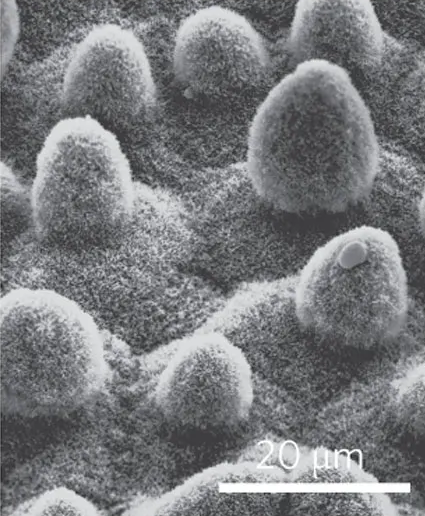
\includegraphics[height=6cm]{lotus.png}
  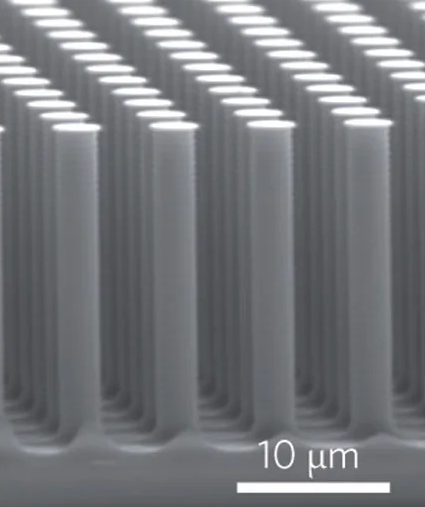
\includegraphics[height=6cm]{micro-pillars.png}
  \caption{(left) Hierarchical structure of a lotus leaf (Nelumbo nucifera). (right) Patterned micro-pillars. Image adapted with permission from \cite{Bocquet}, \textcopyright \enspace Springer Nature.}
  \label{fig:micro-surface}
\end{figure}

From the fluid mechanics perspective, questions invoked by these findings naturally include,
(i) what mechanism leads to the drag reduction, and
(ii) how it can be optimized given other constraints.
The constraints involve surface chemistry, contamination, degradation, fabrication defects, wetting, etc., making the problem truly multiscale and multiphysics.
Basic research along this line, including \emph{Paper 6}, is motivated to resolve at least part of these issues.

Theoretically, the resistance of a solid surface to fluid flows can be characterized by the \emph{slip length}, $\lambda_s$, defined as
\begin{equation}
 \begin{aligned}
  \bm{u}_s = \lambda_s \bigg( \nabla {\bm u} + (\nabla {\bm u})^T \bigg) \cdot \bm{n},
 \end{aligned}
\end{equation}
where $\bm{u}$ is the flow velocity, $\bm{u}_s$ the slip velocity on the solid surface, and $\bm n$ the normal vector pointing from the solid to the fluid.
In the case of a planar simple shear flow, it can be reduced to
\begin{equation}
 \begin{aligned}
  u_s = \lambda_s \dot{\gamma},
 \end{aligned}
\end{equation}
where $\dot{\gamma}=\partial u/\partial y$ is the shear rate.
%This simple relation is also called the Navier slip.
In most situations, $\lambda_s$ is a constant material property with a value on the order-of-magnitude of the molecular interaction range \citep{Thompson_Troian_1997}.
However, even with a no-slip boundary condition, many of the aforementioned studies have demonstrated a large measurable slippage over SHS.
Close inspection of the surface structure suggests that it is the hairy pattern combined with its hydrophobic property that yields the apparent slip.
This is beautifully depicted in Figure \ref{fig:micro-surface}, which shows the natural meadow-looking roughness on a lotus leaf and an artificial array of micron-scale pillars. 

To quantify the slippage analytically, one can define an \emph{effective slip length}, $\lambda_e$, as
\begin{equation} \label{eff slip}
  \lambda_e = \frac{\bar{u}(H)}{\dot{\gamma}}-H,
\end{equation}
where $\bar{u}(H)$ is the average streamwise velocity at a small distance $H$ above the substrate.
Physically, $\lambda_e$ is equal to the distance below the surface at which the velocity would extrapolate to zero.
Under this simple definition, many studies have been conducted to obtaining theoretical expressions of the effective slip for two-dimensional longitudinal or transverse grooves \citep{Lauga_Stone, Sbragalia_Prosperetti, Davis_Lauga, Ng_Wang, Schonecker, Nizkaya, Crowdy_tran, Crowdy_long}.
The general procedure is to solve the Stokes equations in a periodic domain subject to a mixture of no-slip and finite-slip boundary conditions. To facilitate analytical calculations, some simplifications may have to be made, such as a static interface shape and pinning of the contact line.
In general, different geometry- and viscosity-ratio-dependent expressions for $\lambda_e$ have been found, depending on the configuration.

While these solutions are helpful in guiding the optimal surface design, they neglect an important ingredient -- wetting of the fluid.
One reason that superhydrophobic or liquid-infused surfaces are still mostly limited to laboratory testings at present is the various failure modes, often associated with wetting in some form.
Specifically, SHS is known to be sensitive to external pressure under which the entrapped bubble can collapse \citep{Bocquet}; whereas LIS is prone to shear-driven failures, \ie drainage of the lubricant from the surface grooves \citep{Wexler}.
Therefore, the \emph{dynamics} is equally, if not more, important comparing to the static slippage property.
Unfortunately, precise control of wetting in experiments is still very challenging due to sensitivity to surface conditions and instrument inaccuracies \citep{Liu_vuckovac_etal_2019}, let alone the longstanding theoretical disputes \citep{deGennes_wetting}.
In light of these difficulties, numerical studies with controlled parameters in non-ideal situations are expected to bridge the gap between analytical calculations and experimental findings.


\section{Droplets in turbulence}

Turbulence is the unsteady flow generated from the Navier-Stokes equations at large Reynolds numbers.
As it prevails in a broad range of length and time scales, predicting the statistics of droplets or bubbles in turbulence is of great practical importance.
Take the size distribution for example.
In the ocean, air bubbles entrained in breaking waves enhance the air-sea gas flux, affect aerosol production, scavenge biological surfactants, and create ambient noise; knowing their creation mechanism and distribution in size can thus greatly improve our understanding of the nature and climate \citep{deane_stokes_2002a}.
In the atmosphere, vapor condenses on particles and forms droplets; the droplet size distribution is the defining characteristics of a cloud, controlling how it interacts with electromagnetic radiation and how fast precipitation will form \citep{Shaw_2003}.
In emulsions or colloidal suspensions, the distribution of the dispersed phase determines the stability, rheology, and area available for physical or chemical processes that occur at the interface \citep{boxall_etal_2012}. This is directly related to our daily life, as many processed food and cosmetic products are complex fluids in one way or another.

\begin{figure}%[t]
  \centering
  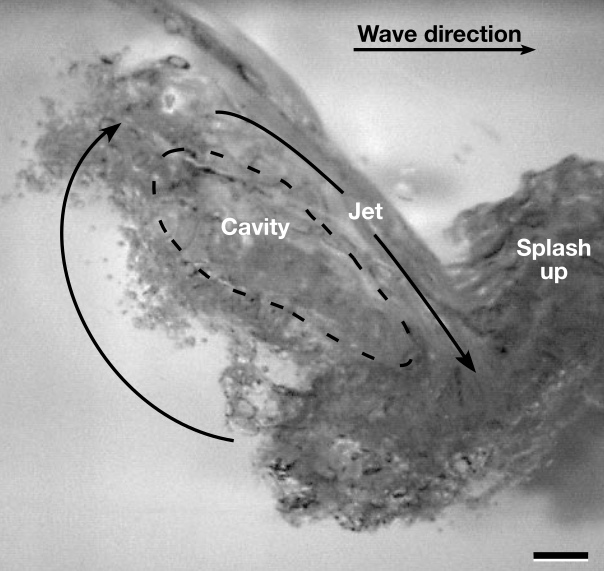
\includegraphics[height=4.57cm]{ocean_wave.png}
  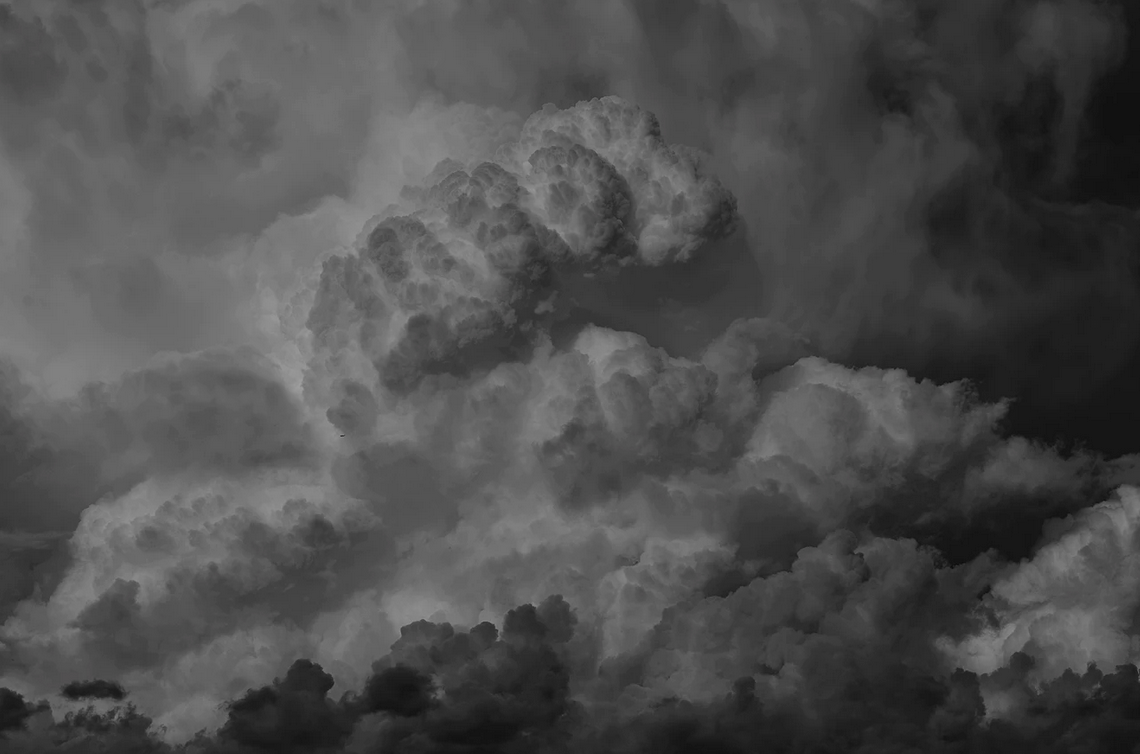
\includegraphics[height=4.57cm]{nimbus_cloud.png}
  \caption{(left) A lab-generated breaking wave crest, showing bubble entrainment. Scale bar, 1 cm. Image adapted with permission from \cite{deane_stokes_2002a}, \textcopyright \enspace Springer Nature. (right) Nimbostratus clouds taken at Karlskrona, Sweden. \textcopyright \enspace Jari Hyt\"onen.}
  \label{fig:wave-cloud}
\end{figure}

Given the ubiquity and importance, detailed numerical simulations on droplet-turbulence interactions are surprisingly scarce. It is not until the last few years that computational studies start to appear in the literature, see \cite{perlekar_biferale_sbragaglia_srivastava_toschi_2012a, skartlien_sollum_schumann_2013a, komrakova_eskin_derksen_2015a, scarbolo_bianco_soldati_2015a, dodd_ferrante_2016a}.
Here, the advantages of performing these large-scale simulations are dual.
On the one hand, interface-resolved, high-resolution simulations reveal a unprecedented level of details, offering arguably the full droplet and flow statistics within the afforded system. These results can then be used as benchmarks to test theoretical scalings and empirical models of the droplet distribution \citep{hinze_1955a, deane_stokes_2002a}.
On the other hand, as simulation methods for multiphase flows are continuously being developed, the current results will serve as verification for later simulations.
Based on these reasons, we performed direct numerical simulations of two immiscible and incompressible fluids in a homogeneous turbulent shear flow under various Weber numbers and initial conditions (\emph{Paper 5}).
The choice of this base flow is rationalized by its natural turbulence sustaining mechanism and the relevance to the logarithmic layer of wall-bounded turbulent flow, see \eg \cite{pumir_1996a, sekimoto_dong_jimenez_2016a}.
We admit that modelling of turbulence is difficult even by itself, let alone in the presence of droplets.
Nevertheless, numerical studies like the one we conducted shall provide additional information to future modellers and shed new lights on the droplet-turbulence interactions.



%===============================================================================
\chapter{Summary}
%===============================================================================






%%===============================================================================
%\chapter{Test chapter, a very very very long title to test the table of contents}
%%===============================================================================
%
%This chapter is meant for testing the correct referencing of figures, equations
%and tables.
%
%% equations
%%
%\begin{equation}
%	1 + 1 = 2
%	\label{eq:test_eq1}
%\end{equation}
%
%\begin{align}
%	2 + 2 = 4
%	\label{eq:test_eq2}
%\end{align}
%
%\begin{equation}
%	3 + 3 = 6
%	\label{eq:test_eq3_intro}
%\end{equation}
%
%% tables
%%
%\begin{table}
%	\centering
%	\begin{tabular}{c}
%		1
%	\end{tabular}
%	\caption{Test table 1}
%	\label{tab:test_tab1}
%\end{table}
%
%\begin{table}
%	\centering
%	\begin{tabular}{c}
%		2
%	\end{tabular}
%	\caption{Test table 2}
%	\label{tab:test_tab2}
%\end{table}
%
%\begin{table}
%	\centering
%	\begin{tabular}{c}
%		3
%	\end{tabular}
%	\caption{Test table 3}
%	\label{tab:test_tab3_intro}
%\end{table}
%
%% figures
%%
%\begin{figure}[h!]
%	\centering
%	test figure 1
%	\caption{Test figure 1}
%	\label{fig:test_fig1}
%\end{figure}
%
%\begin{figure}[h!]
%	\centering
%	test figure 2
%	\caption{Test figure 2}
%	\label{fig:test_fig2}
%\end{figure}
%
%\begin{figure}[h!]
%	\centering
%	test figure 3
%	\caption{Test figure 3}
%	\label{fig:test_fig3_intro}
%\end{figure}
%
%% test references
%%
%\hrule
%\begin{itemize}
%	\item reference to equation 1: \eqref{eq:test_eq1}
%	\item reference to equation 2: \eqref{eq:test_eq2}
%	\item reference to equation 3: \eqref{eq:test_eq3_intro}
%\end{itemize}
%\hrule
%\begin{itemize}
%	\item reference to table 1: \eqref{tab:test_tab1}
%	\item reference to table 2: \eqref{tab:test_tab2}
%	\item reference to table 3: \eqref{tab:test_tab3_intro}
%\end{itemize}
%\hrule
%\begin{itemize}
%	\item reference to figure 1: \eqref{fig:test_fig1}
%	\item reference to figure 2: \eqref{fig:test_fig2}
%	\item reference to figure 3: \eqref{fig:test_fig3_intro}
%\end{itemize}
%\hrule

%===============================================================================
% Acknowledgments
%===============================================================================
%
\begin{acknowledgements}
%  Advisors,
%  funders,
%  collaborators,
%  mentors,
%  colleagues,
%  friends,
%  family.

  The first part of this thesis was written from December 2019 to January 2020, during the warmest winter since I arrived in Stockholm five years ago.
  Looking back, I have encountered, experienced and learned so much from uncountable people that is nearly impossible to name them one by one.
  I am grateful to \emph{everyone} and apologize in advance for any negligence.

  First and foremost, I thank Professor Luca Brandt for accepting me in and guiding me through the PhD program at KTH Mechanics.
  His strong leadership from the inception,
  enthusiastic responses and constructive criticisms at every discussion,
  generous support and increasing trust in me towards the end are indispensable for me to grow and develop academically.
  For these reasons, I owe my deepest gratitude to him.

  Second, I wish to extend my sincere thanks to my day-to-day advisors and mentors at KTH.
  I thank Outi Tammisolar for co-advising me since my first project, following my progress throughout the PhD
  and offering me invaluable career advice in the later years.
  I thank Jean-Christophe Loiseau for instilling in me the European culture, proper programming and mathematical rigour.
  I also thank Mehdi Niazi for always being available for technical discussions or code debugging and sharing his wisdom whenever I am lost.
  The patience, support and encouragement they offered me are instrumental in building my confidence and independence, which I will never take for granted.

  Third, I want to express my appreciation to all collaborators and senior colleagues that have shaped and contributed to my PhD work.
  These include, but are not limited to, international collaborators: Michael Dodd, Alexander Leshansky, Itzhak Fouxon and Naoki Takeishi;
  former and present colleagues at KTH: Walter Fornari, Pedro Costa, Francesco de Vita, Marco Rosti, B. M. Ningegowda and U\'{g}is L\={a}cis;
  office mates: Ricardo Vinuesa, Ekaterina Ezhova, Tímea Kékesi, Arash Alizad Banaei and Ashwin Vishnu;
  and professors that I enjoy talking to or playing innebandy with:
  Shervin Bagheri, Christophe Duwig, Hanno Essén, Nicholas Apazidis, Lanie Gutierrez-Farewik and Fredrik Lundell.
  Many others have also helped, corrected or inspired me in various research projects;
  my thanks are expressed in the separate acknowledgements after each paper in the next part of the thesis.
  
  In his famous essay, \emph{\small The World As I See It}, Einstein wrote,
  ``But from the point of view of daily life, without going deeper, we exist for our fellowmen --
  in the first place for those on whose smiles and welfare all our happiness depends,
  and next for all those unknown to us personally with whose destinies we are bound up by the tie of sympathy.''
  In the last several years, I have been lucky to derive plentiful happiness and sympathy from Artem, Erik, Guillaume, Nicolas, Frida, Natasha, Thea, Lee,
  as well as the rest of the Roslagstullsbacken corridor.
  Particularly, I am blessed to meet Dia, whose courage, ambition, curiosity and sensitivity have become a continuing source of my attachment,
  making me feel thorough and complete.
  
  Finally, none of the above would have been possible without the enduring love, hope, protection and education from my family at home.
  
  \chinese{爸,妈}
  
  \chinese{感谢你们对我从小到大的培养}

  \chinese{感谢你们对我的一切付出}

  \chinese{我的所有都属于你们}
  
  
\end{acknowledgements}



%===============================================================================
% References
%===============================================================================
%
\bibliographystyle{jfm}
\bibliography{thesis}
%
\IfFileExists{overview.bbl}{\graphicspath{{imgs/}}

%===============================================================================
\chapter{Introduction}
%===============================================================================



In \cite{Batchelor} we believe.


%-------------------------------------------------------------------------------

\section{Flow-assist droplet assembly}

material science,
photonic crystals,
microfluidics,
lab-on-a-chip.


\section{Liquid-infused surfaces}

drag reduction,
surface engineering,
superhydrophobicity,
lubricant-infused surfaces.


\section{Suspension flows}

particle suspensions,
complex fluids,
rheology,
shear thickening.

\thesisstructure Add here a brief description of the structure of the thesis.



%===============================================================================
\chapter{Microhydrodynamics}
%===============================================================================


In this chapter, we give a brief theoretical background of the topics studied.

mention the abuse of terms between droplets and particles.

The incompressible Navier-Stokes equation
\begin{subequations}
 \begin{equation}
   \nabla \cdot {\bm u} = 0,
  \label{eq:div-free}
 \end{equation}
 \begin{equation}
   \rho \bigg(\frac{\partial {\bm u}}{\partial t} + {\bm u} \cdot \nabla {\bm u} \bigg) = -\nabla p + \mu \nabla ^2  {\bm u} + {\bm f},
  \label{eq:NS}
 \end{equation}
\end{subequations}
governs the dynamics of Newtonian fluids (which is what we consider throughout the thesis).
where...

boundary conditions... between fluid and solid: continuity of the tangential velocity, \ie the no-slip condition (molecular slip ignored).
with an interface... surface tension... free surface... a boundary condition for the stress (see \cite{Batchelor} Sec.\ 3.3).


the Reynolds, Weber, and Froude numbers, defined as
\begin{equation}
  \begin{aligned}
    Re = \frac{\tilde{\rho} \tilde{U} \tilde{L}}{\tilde{\mu}},\quad \quad We = \frac{\tilde{\rho} \tilde{U}^2 \tilde{L}}{\tilde{\sigma}},\quad \quad Fr=\frac{\tilde{U}^2}{\tilde{g}\tilde{L}},      
  \label{eq:non-di-num}    
  \end{aligned}
\end{equation}
\noindent where $\tilde{U}$, $\tilde{L}$, $\tilde{\rho_1}$, $\tilde{\mu_1}$, and $\tilde{g}$ denote the reference dimensional velocity, length, density, dynamic viscosity, and gravitational acceleration. Note that $\rho_1=1$ and $\mu_1=1$ (i.e.\ we define fluid 1 as the reference fluid).
Perhaps also mention the Stouhal number.



%-------------------------------------------------------------------------------

\section{Stokes flow and its symmetries}

When small Reynolds number, Eq.\ \eqref{eq:NS} reduces to the Stokes equation,
\begin{equation}
   -\nabla p + \mu \nabla ^2  {\bm u} + {\bm f} = {\bm 0},
 \label{eq:Stokes}
\end{equation}
or, equivalently
\begin{equation}
   \nabla \cdot  {\bm \sigma} + {\bm f} = {\bm 0},
 \label{eq:Stokes1}
\end{equation}
where...

Stokes flow has the following symmetries and properties.
\begin{enumerate}
 \item \emph{Linearity}, which renders the applicability of superposition principle. For example, if $({\bm u}_1,p_1)$ is a solution to ${\bm f}={\bm f}_1$ and $({\bm u}_2,p_2)$ is a solution to ${\bm f}={\bm f}_2$, then $(\alpha{\bm u}_1+\beta {\bm u}_2,\alpha p_1 + \beta p_2)$ is a solution to ${\bm f}=\alpha{\bm f}_1 + \beta {\bm f}_2$.
 \item \emph{Reversibility}, which follows from the linearity and entails that, if the forcing changes from ${\bm f}$ to $-{\bm f}$, then the flow should reverse, \ie $({\bm u},p) \to (-{\bm u},-p)$. Note that, the simple reversibility symmetry can be very useful in deducing qualitative results without doing any calulation, see \eg the much celebrated note of \cite{Purcell1977}
 \item \emph{Stress equilibrium}, which states that any force exerted within the fluid is transmitted instantaneously to the boundary or, if there is no boundary, to infinity \citep{graham_2018}.
 \item \emph{Lorentz reciprocal relation}, which relates two solutions, $({\bm u}', {\bm \sigma}')$ and $({\bm u}'', {\bm \sigma}'')$ (they may differ by boundary conditions), of the Stokes equation by,
 \begin{equation}
  \small
  \begin{aligned}
   \int_V \bigg({\bm u}' \cdot (\nabla  \cdot {\bm \sigma}'') - {\bm u}'' \cdot (\nabla  \cdot {\bm \sigma}')\bigg) dV  & =\\
   \int_S \bigg({\bm u}' \cdot ({\bm n} \cdot {\bm \sigma}'') - {\bm u}'' \cdot ({\bm n} \cdot {\bm \sigma}')\bigg) dS, & 
  \end{aligned} \label{eq:lorentz-recip}
 \end{equation}
 where $V$ is some enclosed volume with surface $S$.
 \item \emph{Minimum dissipation principle}, which is a variational principle that asserts that the flow that minimizes energy dissipation rate subject to incompressibility and certain boundary conditions is the Stokes flow in that geometry.
\end{enumerate}


\section{Single particle in Stokes flow}

Green's function (Stoekslet),
stresslet (symmetric and traceless),
scaling laws (decay),
Fax\'{e}n's law,
confinement,
multipole expansion,
boundary integral methods.


\section{Particle interactions}

Batchelor and Green (1972),
swapping,
dancing,
range of interactions,
dipolar theory,
lubrication approximation.


\section{Rheology}

microstructure,
many-body problems (theoretical difficulties),
macroscopic properties, averages and bulk stresses (see Brady and Bossis).

The behaviour of systems involving the motion of small particles relative to a suspending fluid covers a wide range of phenomena of interest to both scientists and engineers. Dense suspensions, where the volume fraction of solid particles becomes comparable to or even higher than that of the fluid (see Figure \ref{fig:snap}), have particularly rich and sometimes unexpected rheologies, such as yielding, shear thinning, continuous shear thickening (CST), or discontinuous shear thickening (DST) \citep{mewis_wagner_book, Morton_Morris_2014, guazzelli_pouliquen_2018, Morris_annurev2020}. Apart from being theoretically intriguing, these complex behaviours often have major implications in practice. For instance, while it makes sense for the cement industry to manufacture suspensions that do not shear thicken, the same feature becomes an advantage for designing flexible body armor.



%===============================================================================
\chapter{Numerical Methods}
%===============================================================================



limitation of theoretical approaches,
necessity of numerical solutions.

Despite the practical importance, theoretical development of suspension rheology remains chanllenging and only a few analytical solutions have been found in the dilute regime, see \eg \cite{Einstein_1906, batchelor_green_1972b}. This is partially due to a lack of precise knowledge or control of various interactions at the particle level, partially due to the mathematical difficulties involved in many-body problems. On the other hand, solving a system of interacting particles is relatively straightforward in an algorithmic perspective. In fact, the last decades have seen tremendous advancement in both numerical simulations and computer hardware.

governing equations.

numerical solutions.


%-------------------------------------------------------------------------------

\section{Fluid-resolved methods}

level set methods,
(interface-correction level set/ghost fluid method),
volume-of-fluid methods,
phase-field methods,
immersed boundary methods.


\section{Particle-based methods}

The central equation to solve is
\begin{equation} 
 \begin{aligned} \label{eq:force-balance}
  {\bm m} \cdot \frac{d{\bm U}}{dt} = {\bm F}^H + {\bm F}^P, 
 \end{aligned}
\end{equation}
where ${\bm m}$ is a generalized mass/moment-of-inertia matrix of dimension $6N \times 6N$,
${\bm U}$ is the particle translational/rotational velocity vector of dimension $6N$,
and ${\bm F}$ represent the $6N$ force/torque vectors owing to hydrodynamics (denoted with superscript $\footnotesize H$) or other interactions (denoted with superscript $\footnotesize P$). Specifically, ${\bm F}^P$ may include contact, electrostatic, van der Waars, or magnetic forces, \etc. In principle, stochastic forces can also be included in the general formulation, though its numerical treatments demand special care such that fluctuation-dissipation theorem is satified. In the present thesis, Brownian motions are neglected.

For inertialess particles in Stokes flow, the task is to solve Eq.\ \eqref{eq:force-balance} subject to ${\bm m} \cdot (d{\bm U}/dt) \to 0$. Various techniques exist as summarized below.

\subsection{Stokesian dynamics}

The Stokesian dynamics \citep{Brady_Bossis1988} employs the fact that, when the particle Reynolds number is small and the bulk flow is linear, the hydrodynamic forces and stresses exerted on the particles by the fluid can be expressed as
\begin{equation} 
 \begin{aligned} \label{eq:sd-hydro}
  \begin{pmatrix}
   {\bm F}^H \\
   {\bm S}^H
  \end{pmatrix}
  = - \mathscr{R} \cdot
  \begin{pmatrix}
   {\bm U}-{\bm U}^\infty \\
   -{\bm E}^\infty
  \end{pmatrix},
 \end{aligned}
\end{equation}
where
\begin{equation} 
 \begin{aligned}
  \mathscr{R} =
  \begin{pmatrix}
   {\bm R}_{FU} & {\bm R}_{FE} \\
   {\bm R}_{SU} & {\bm R}_{SE}
  \end{pmatrix},
 \end{aligned}
\end{equation}
is termed the ``grand resistance'' matrix. 
If $\mathscr{R}$ is known, 
formulate the problem as

It is calculated as
\begin{equation} 
 \begin{aligned}
  \mathscr{R} = (\mathscr{M}^\infty)^{-1} +\mathscr{R}_{2B} - \mathscr{R}_{2B}^\infty.
 \end{aligned}
\end{equation}          
Es.\ \eqref{eq:sd-hydro} is then inverted and integrated in time to obtain the dynamics.


\subsection{Dissipative particle dynamics}

dissipative particle dynamics (DPD) \citep{Hoogerbrugge_1992, Groot_Warren_1997}


\subsection{Discrete element methods}


discrete element methods (DEM) \citep{Mari_Seto_2014JoR, Cheal_Ness_2018}, to name a few.
 the discrete-element lubrication/contact dynamics (DLCD) model.




%===============================================================================
\chapter{Summary}
%===============================================================================






%%===============================================================================
%\chapter{Test chapter, a very very very long title to test the table of contents}
%%===============================================================================
%
%This chapter is meant for testing the correct referencing of figures, equations
%and tables.
%
%% equations
%%
%\begin{equation}
%	1 + 1 = 2
%	\label{eq:test_eq1}
%\end{equation}
%
%\begin{align}
%	2 + 2 = 4
%	\label{eq:test_eq2}
%\end{align}
%
%\begin{equation}
%	3 + 3 = 6
%	\label{eq:test_eq3_intro}
%\end{equation}
%
%% tables
%%
%\begin{table}
%	\centering
%	\begin{tabular}{c}
%		1
%	\end{tabular}
%	\caption{Test table 1}
%	\label{tab:test_tab1}
%\end{table}
%
%\begin{table}
%	\centering
%	\begin{tabular}{c}
%		2
%	\end{tabular}
%	\caption{Test table 2}
%	\label{tab:test_tab2}
%\end{table}
%
%\begin{table}
%	\centering
%	\begin{tabular}{c}
%		3
%	\end{tabular}
%	\caption{Test table 3}
%	\label{tab:test_tab3_intro}
%\end{table}
%
%% figures
%%
%\begin{figure}[h!]
%	\centering
%	test figure 1
%	\caption{Test figure 1}
%	\label{fig:test_fig1}
%\end{figure}
%
%\begin{figure}[h!]
%	\centering
%	test figure 2
%	\caption{Test figure 2}
%	\label{fig:test_fig2}
%\end{figure}
%
%\begin{figure}[h!]
%	\centering
%	test figure 3
%	\caption{Test figure 3}
%	\label{fig:test_fig3_intro}
%\end{figure}
%
%% test references
%%
%\hrule
%\begin{itemize}
%	\item reference to equation 1: \eqref{eq:test_eq1}
%	\item reference to equation 2: \eqref{eq:test_eq2}
%	\item reference to equation 3: \eqref{eq:test_eq3_intro}
%\end{itemize}
%\hrule
%\begin{itemize}
%	\item reference to table 1: \eqref{tab:test_tab1}
%	\item reference to table 2: \eqref{tab:test_tab2}
%	\item reference to table 3: \eqref{tab:test_tab3_intro}
%\end{itemize}
%\hrule
%\begin{itemize}
%	\item reference to figure 1: \eqref{fig:test_fig1}
%	\item reference to figure 2: \eqref{fig:test_fig2}
%	\item reference to figure 3: \eqref{fig:test_fig3_intro}
%\end{itemize}
%\hrule

%===============================================================================
% Acknowledgments
%===============================================================================
%
\begin{acknowledgements}
%  Advisors,
%  funders,
%  collaborators,
%  mentors,
%  colleagues,
%  friends,
%  family.

  The first part of this thesis was written from December 2019 to January 2020, during the warmest winter since I arrived in Stockholm five years ago.
  Looking back, I have encountered, experienced and learned so much from uncountable people that is nearly impossible to name them one by one.
  I am grateful to \emph{everyone} and apologize in advance for any negligence.

  First and foremost, I thank Professor Luca Brandt for accepting me in and guiding me through the PhD program at KTH Mechanics.
  His strong leadership from the inception,
  enthusiastic responses and constructive criticisms at every discussion,
  generous support and increasing trust in me towards the end are indispensable for me to grow and develop academically.
  For these reasons, I owe my deepest gratitude to him.

  Second, I wish to extend my sincere thanks to my day-to-day advisors and mentors at KTH.
  I thank Outi Tammisolar for co-advising me since my first project, following my progress throughout the PhD
  and offering me invaluable career advice in the later years.
  I thank Jean-Christophe Loiseau for instilling in me the European culture, proper programming and mathematical rigour.
  I also thank Mehdi Niazi for always being available for technical discussions or code debugging and sharing his wisdom whenever I am lost.
  The patience, support and encouragement they offered me are instrumental in building my confidence and independence, which I will never take for granted.

  Third, I want to express my appreciation to all collaborators and senior colleagues that have shaped and contributed to my PhD work.
  These include, but are not limited to, international collaborators: Michael Dodd, Alexander Leshansky, Itzhak Fouxon and Naoki Takeishi;
  former and present colleagues at KTH: Walter Fornari, Pedro Costa, Francesco de Vita, Marco Rosti, B. M. Ningegowda and U\'{g}is L\={a}cis;
  office mates: Ricardo Vinuesa, Ekaterina Ezhova, Tímea Kékesi, Arash Alizad Banaei and Ashwin Vishnu;
  and professors that I enjoy talking to or playing innebandy with:
  Shervin Bagheri, Christophe Duwig, Hanno Essén, Nicholas Apazidis, Lanie Gutierrez-Farewik and Fredrik Lundell.
  Many others have also helped, corrected or inspired me in various research projects;
  my thanks are expressed in the separate acknowledgements after each paper in the next part of the thesis.
  
  In his famous essay, \emph{\small The World As I See It}, Einstein wrote,
  ``But from the point of view of daily life, without going deeper, we exist for our fellowmen --
  in the first place for those on whose smiles and welfare all our happiness depends,
  and next for all those unknown to us personally with whose destinies we are bound up by the tie of sympathy.''
  In the last several years, I have been lucky to derive plentiful happiness and sympathy from Artem, Erik, Guillaume, Nicolas, Frida, Natasha, Thea, Lee,
  as well as the rest of the Roslagstullsbacken corridor.
  Particularly, I am blessed to meet Dia, whose courage, ambition, curiosity and sensitivity have become a continuing source of my attachment,
  making me feel thorough and complete.
  
  Finally, none of the above would have been possible without the enduring love, hope, protection and education from my family at home.
  
  \chinese{爸,妈}
  
  \chinese{感谢你们对我从小到大的培养}

  \chinese{感谢你们对我的一切付出}

  \chinese{我的所有都属于你们}
  
  
\end{acknowledgements}



%===============================================================================
% References
%===============================================================================
%
\bibliographystyle{jfm}
\bibliography{thesis}
%
\IfFileExists{overview.bbl}{\graphicspath{{imgs/}}

%===============================================================================
\chapter{Introduction}
%===============================================================================



In \cite{Batchelor} we believe.


%-------------------------------------------------------------------------------

\section{Flow-assist droplet assembly}

material science,
photonic crystals,
microfluidics,
lab-on-a-chip.


\section{Liquid-infused surfaces}

drag reduction,
surface engineering,
superhydrophobicity,
lubricant-infused surfaces.


\section{Suspension flows}

particle suspensions,
complex fluids,
rheology,
shear thickening.

\thesisstructure Add here a brief description of the structure of the thesis.



%===============================================================================
\chapter{Microhydrodynamics}
%===============================================================================


In this chapter, we give a brief theoretical background of the topics studied.

mention the abuse of terms between droplets and particles.

The incompressible Navier-Stokes equation
\begin{subequations}
 \begin{equation}
   \nabla \cdot {\bm u} = 0,
  \label{eq:div-free}
 \end{equation}
 \begin{equation}
   \rho \bigg(\frac{\partial {\bm u}}{\partial t} + {\bm u} \cdot \nabla {\bm u} \bigg) = -\nabla p + \mu \nabla ^2  {\bm u} + {\bm f},
  \label{eq:NS}
 \end{equation}
\end{subequations}
governs the dynamics of Newtonian fluids (which is what we consider throughout the thesis).
where...

boundary conditions... between fluid and solid: continuity of the tangential velocity, \ie the no-slip condition (molecular slip ignored).
with an interface... surface tension... free surface... a boundary condition for the stress (see \cite{Batchelor} Sec.\ 3.3).


the Reynolds, Weber, and Froude numbers, defined as
\begin{equation}
  \begin{aligned}
    Re = \frac{\tilde{\rho} \tilde{U} \tilde{L}}{\tilde{\mu}},\quad \quad We = \frac{\tilde{\rho} \tilde{U}^2 \tilde{L}}{\tilde{\sigma}},\quad \quad Fr=\frac{\tilde{U}^2}{\tilde{g}\tilde{L}},      
  \label{eq:non-di-num}    
  \end{aligned}
\end{equation}
\noindent where $\tilde{U}$, $\tilde{L}$, $\tilde{\rho_1}$, $\tilde{\mu_1}$, and $\tilde{g}$ denote the reference dimensional velocity, length, density, dynamic viscosity, and gravitational acceleration. Note that $\rho_1=1$ and $\mu_1=1$ (i.e.\ we define fluid 1 as the reference fluid).
Perhaps also mention the Stouhal number.



%-------------------------------------------------------------------------------

\section{Stokes flow and its symmetries}

When small Reynolds number, Eq.\ \eqref{eq:NS} reduces to the Stokes equation,
\begin{equation}
   -\nabla p + \mu \nabla ^2  {\bm u} + {\bm f} = {\bm 0},
 \label{eq:Stokes}
\end{equation}
or, equivalently
\begin{equation}
   \nabla \cdot  {\bm \sigma} + {\bm f} = {\bm 0},
 \label{eq:Stokes1}
\end{equation}
where...

Stokes flow has the following symmetries and properties.
\begin{enumerate}
 \item \emph{Linearity}, which renders the applicability of superposition principle. For example, if $({\bm u}_1,p_1)$ is a solution to ${\bm f}={\bm f}_1$ and $({\bm u}_2,p_2)$ is a solution to ${\bm f}={\bm f}_2$, then $(\alpha{\bm u}_1+\beta {\bm u}_2,\alpha p_1 + \beta p_2)$ is a solution to ${\bm f}=\alpha{\bm f}_1 + \beta {\bm f}_2$.
 \item \emph{Reversibility}, which follows from the linearity and entails that, if the forcing changes from ${\bm f}$ to $-{\bm f}$, then the flow should reverse, \ie $({\bm u},p) \to (-{\bm u},-p)$. Note that, the simple reversibility symmetry can be very useful in deducing qualitative results without doing any calulation, see \eg the much celebrated note of \cite{Purcell1977}
 \item \emph{Stress equilibrium}, which states that any force exerted within the fluid is transmitted instantaneously to the boundary or, if there is no boundary, to infinity \citep{graham_2018}.
 \item \emph{Lorentz reciprocal relation}, which relates two solutions, $({\bm u}', {\bm \sigma}')$ and $({\bm u}'', {\bm \sigma}'')$ (they may differ by boundary conditions), of the Stokes equation by,
 \begin{equation}
  \small
  \begin{aligned}
   \int_V \bigg({\bm u}' \cdot (\nabla  \cdot {\bm \sigma}'') - {\bm u}'' \cdot (\nabla  \cdot {\bm \sigma}')\bigg) dV  & =\\
   \int_S \bigg({\bm u}' \cdot ({\bm n} \cdot {\bm \sigma}'') - {\bm u}'' \cdot ({\bm n} \cdot {\bm \sigma}')\bigg) dS, & 
  \end{aligned} \label{eq:lorentz-recip}
 \end{equation}
 where $V$ is some enclosed volume with surface $S$.
 \item \emph{Minimum dissipation principle}, which is a variational principle that asserts that the flow that minimizes energy dissipation rate subject to incompressibility and certain boundary conditions is the Stokes flow in that geometry.
\end{enumerate}


\section{Single particle in Stokes flow}

Green's function (Stoekslet),
stresslet (symmetric and traceless),
scaling laws (decay),
Fax\'{e}n's law,
confinement,
multipole expansion,
boundary integral methods.


\section{Particle interactions}

Batchelor and Green (1972),
swapping,
dancing,
range of interactions,
dipolar theory,
lubrication approximation.


\section{Rheology}

microstructure,
many-body problems (theoretical difficulties),
macroscopic properties, averages and bulk stresses (see Brady and Bossis).

The behaviour of systems involving the motion of small particles relative to a suspending fluid covers a wide range of phenomena of interest to both scientists and engineers. Dense suspensions, where the volume fraction of solid particles becomes comparable to or even higher than that of the fluid (see Figure \ref{fig:snap}), have particularly rich and sometimes unexpected rheologies, such as yielding, shear thinning, continuous shear thickening (CST), or discontinuous shear thickening (DST) \citep{mewis_wagner_book, Morton_Morris_2014, guazzelli_pouliquen_2018, Morris_annurev2020}. Apart from being theoretically intriguing, these complex behaviours often have major implications in practice. For instance, while it makes sense for the cement industry to manufacture suspensions that do not shear thicken, the same feature becomes an advantage for designing flexible body armor.



%===============================================================================
\chapter{Numerical Methods}
%===============================================================================



limitation of theoretical approaches,
necessity of numerical solutions.

Despite the practical importance, theoretical development of suspension rheology remains chanllenging and only a few analytical solutions have been found in the dilute regime, see \eg \cite{Einstein_1906, batchelor_green_1972b}. This is partially due to a lack of precise knowledge or control of various interactions at the particle level, partially due to the mathematical difficulties involved in many-body problems. On the other hand, solving a system of interacting particles is relatively straightforward in an algorithmic perspective. In fact, the last decades have seen tremendous advancement in both numerical simulations and computer hardware.

governing equations.

numerical solutions.


%-------------------------------------------------------------------------------

\section{Fluid-resolved methods}

level set methods,
(interface-correction level set/ghost fluid method),
volume-of-fluid methods,
phase-field methods,
immersed boundary methods.


\section{Particle-based methods}

The central equation to solve is
\begin{equation} 
 \begin{aligned} \label{eq:force-balance}
  {\bm m} \cdot \frac{d{\bm U}}{dt} = {\bm F}^H + {\bm F}^P, 
 \end{aligned}
\end{equation}
where ${\bm m}$ is a generalized mass/moment-of-inertia matrix of dimension $6N \times 6N$,
${\bm U}$ is the particle translational/rotational velocity vector of dimension $6N$,
and ${\bm F}$ represent the $6N$ force/torque vectors owing to hydrodynamics (denoted with superscript $\footnotesize H$) or other interactions (denoted with superscript $\footnotesize P$). Specifically, ${\bm F}^P$ may include contact, electrostatic, van der Waars, or magnetic forces, \etc. In principle, stochastic forces can also be included in the general formulation, though its numerical treatments demand special care such that fluctuation-dissipation theorem is satified. In the present thesis, Brownian motions are neglected.

For inertialess particles in Stokes flow, the task is to solve Eq.\ \eqref{eq:force-balance} subject to ${\bm m} \cdot (d{\bm U}/dt) \to 0$. Various techniques exist as summarized below.

\subsection{Stokesian dynamics}

The Stokesian dynamics \citep{Brady_Bossis1988} employs the fact that, when the particle Reynolds number is small and the bulk flow is linear, the hydrodynamic forces and stresses exerted on the particles by the fluid can be expressed as
\begin{equation} 
 \begin{aligned} \label{eq:sd-hydro}
  \begin{pmatrix}
   {\bm F}^H \\
   {\bm S}^H
  \end{pmatrix}
  = - \mathscr{R} \cdot
  \begin{pmatrix}
   {\bm U}-{\bm U}^\infty \\
   -{\bm E}^\infty
  \end{pmatrix},
 \end{aligned}
\end{equation}
where
\begin{equation} 
 \begin{aligned}
  \mathscr{R} =
  \begin{pmatrix}
   {\bm R}_{FU} & {\bm R}_{FE} \\
   {\bm R}_{SU} & {\bm R}_{SE}
  \end{pmatrix},
 \end{aligned}
\end{equation}
is termed the ``grand resistance'' matrix. 
If $\mathscr{R}$ is known, 
formulate the problem as

It is calculated as
\begin{equation} 
 \begin{aligned}
  \mathscr{R} = (\mathscr{M}^\infty)^{-1} +\mathscr{R}_{2B} - \mathscr{R}_{2B}^\infty.
 \end{aligned}
\end{equation}          
Es.\ \eqref{eq:sd-hydro} is then inverted and integrated in time to obtain the dynamics.


\subsection{Dissipative particle dynamics}

dissipative particle dynamics (DPD) \citep{Hoogerbrugge_1992, Groot_Warren_1997}


\subsection{Discrete element methods}


discrete element methods (DEM) \citep{Mari_Seto_2014JoR, Cheal_Ness_2018}, to name a few.
 the discrete-element lubrication/contact dynamics (DLCD) model.




%===============================================================================
\chapter{Summary}
%===============================================================================






%%===============================================================================
%\chapter{Test chapter, a very very very long title to test the table of contents}
%%===============================================================================
%
%This chapter is meant for testing the correct referencing of figures, equations
%and tables.
%
%% equations
%%
%\begin{equation}
%	1 + 1 = 2
%	\label{eq:test_eq1}
%\end{equation}
%
%\begin{align}
%	2 + 2 = 4
%	\label{eq:test_eq2}
%\end{align}
%
%\begin{equation}
%	3 + 3 = 6
%	\label{eq:test_eq3_intro}
%\end{equation}
%
%% tables
%%
%\begin{table}
%	\centering
%	\begin{tabular}{c}
%		1
%	\end{tabular}
%	\caption{Test table 1}
%	\label{tab:test_tab1}
%\end{table}
%
%\begin{table}
%	\centering
%	\begin{tabular}{c}
%		2
%	\end{tabular}
%	\caption{Test table 2}
%	\label{tab:test_tab2}
%\end{table}
%
%\begin{table}
%	\centering
%	\begin{tabular}{c}
%		3
%	\end{tabular}
%	\caption{Test table 3}
%	\label{tab:test_tab3_intro}
%\end{table}
%
%% figures
%%
%\begin{figure}[h!]
%	\centering
%	test figure 1
%	\caption{Test figure 1}
%	\label{fig:test_fig1}
%\end{figure}
%
%\begin{figure}[h!]
%	\centering
%	test figure 2
%	\caption{Test figure 2}
%	\label{fig:test_fig2}
%\end{figure}
%
%\begin{figure}[h!]
%	\centering
%	test figure 3
%	\caption{Test figure 3}
%	\label{fig:test_fig3_intro}
%\end{figure}
%
%% test references
%%
%\hrule
%\begin{itemize}
%	\item reference to equation 1: \eqref{eq:test_eq1}
%	\item reference to equation 2: \eqref{eq:test_eq2}
%	\item reference to equation 3: \eqref{eq:test_eq3_intro}
%\end{itemize}
%\hrule
%\begin{itemize}
%	\item reference to table 1: \eqref{tab:test_tab1}
%	\item reference to table 2: \eqref{tab:test_tab2}
%	\item reference to table 3: \eqref{tab:test_tab3_intro}
%\end{itemize}
%\hrule
%\begin{itemize}
%	\item reference to figure 1: \eqref{fig:test_fig1}
%	\item reference to figure 2: \eqref{fig:test_fig2}
%	\item reference to figure 3: \eqref{fig:test_fig3_intro}
%\end{itemize}
%\hrule

%===============================================================================
% Acknowledgments
%===============================================================================
%
\begin{acknowledgements}
%  Advisors,
%  funders,
%  collaborators,
%  mentors,
%  colleagues,
%  friends,
%  family.

  The first part of this thesis was written from December 2019 to January 2020, during the warmest winter since I arrived in Stockholm five years ago.
  Looking back, I have encountered, experienced and learned so much from uncountable people that is nearly impossible to name them one by one.
  I am grateful to \emph{everyone} and apologize in advance for any negligence.

  First and foremost, I thank Professor Luca Brandt for accepting me in and guiding me through the PhD program at KTH Mechanics.
  His strong leadership from the inception,
  enthusiastic responses and constructive criticisms at every discussion,
  generous support and increasing trust in me towards the end are indispensable for me to grow and develop academically.
  For these reasons, I owe my deepest gratitude to him.

  Second, I wish to extend my sincere thanks to my day-to-day advisors and mentors at KTH.
  I thank Outi Tammisolar for co-advising me since my first project, following my progress throughout the PhD
  and offering me invaluable career advice in the later years.
  I thank Jean-Christophe Loiseau for instilling in me the European culture, proper programming and mathematical rigour.
  I also thank Mehdi Niazi for always being available for technical discussions or code debugging and sharing his wisdom whenever I am lost.
  The patience, support and encouragement they offered me are instrumental in building my confidence and independence, which I will never take for granted.

  Third, I want to express my appreciation to all collaborators and senior colleagues that have shaped and contributed to my PhD work.
  These include, but are not limited to, international collaborators: Michael Dodd, Alexander Leshansky, Itzhak Fouxon and Naoki Takeishi;
  former and present colleagues at KTH: Walter Fornari, Pedro Costa, Francesco de Vita, Marco Rosti, B. M. Ningegowda and U\'{g}is L\={a}cis;
  office mates: Ricardo Vinuesa, Ekaterina Ezhova, Tímea Kékesi, Arash Alizad Banaei and Ashwin Vishnu;
  and professors that I enjoy talking to or playing innebandy with:
  Shervin Bagheri, Christophe Duwig, Hanno Essén, Nicholas Apazidis, Lanie Gutierrez-Farewik and Fredrik Lundell.
  Many others have also helped, corrected or inspired me in various research projects;
  my thanks are expressed in the separate acknowledgements after each paper in the next part of the thesis.
  
  In his famous essay, \emph{\small The World As I See It}, Einstein wrote,
  ``But from the point of view of daily life, without going deeper, we exist for our fellowmen --
  in the first place for those on whose smiles and welfare all our happiness depends,
  and next for all those unknown to us personally with whose destinies we are bound up by the tie of sympathy.''
  In the last several years, I have been lucky to derive plentiful happiness and sympathy from Artem, Erik, Guillaume, Nicolas, Frida, Natasha, Thea, Lee,
  as well as the rest of the Roslagstullsbacken corridor.
  Particularly, I am blessed to meet Dia, whose courage, ambition, curiosity and sensitivity have become a continuing source of my attachment,
  making me feel thorough and complete.
  
  Finally, none of the above would have been possible without the enduring love, hope, protection and education from my family at home.
  
  \chinese{爸,妈}
  
  \chinese{感谢你们对我从小到大的培养}

  \chinese{感谢你们对我的一切付出}

  \chinese{我的所有都属于你们}
  
  
\end{acknowledgements}



%===============================================================================
% References
%===============================================================================
%
\bibliographystyle{jfm}
\bibliography{thesis}
%
\IfFileExists{overview.bbl}{\graphicspath{{imgs/}}

%===============================================================================
\chapter{Introduction}
%===============================================================================



In \cite{Batchelor} we believe.


%-------------------------------------------------------------------------------

\section{Flow-assist droplet assembly}

material science,
photonic crystals,
microfluidics,
lab-on-a-chip.


\section{Liquid-infused surfaces}

drag reduction,
surface engineering,
superhydrophobicity,
lubricant-infused surfaces.


\section{Suspension flows}

particle suspensions,
complex fluids,
rheology,
shear thickening.

\thesisstructure Add here a brief description of the structure of the thesis.



%===============================================================================
\chapter{Microhydrodynamics}
%===============================================================================


In this chapter, we give a brief theoretical background of the topics studied.

mention the abuse of terms between droplets and particles.

The incompressible Navier-Stokes equation
\begin{subequations}
 \begin{equation}
   \nabla \cdot {\bm u} = 0,
  \label{eq:div-free}
 \end{equation}
 \begin{equation}
   \rho \bigg(\frac{\partial {\bm u}}{\partial t} + {\bm u} \cdot \nabla {\bm u} \bigg) = -\nabla p + \mu \nabla ^2  {\bm u} + {\bm f},
  \label{eq:NS}
 \end{equation}
\end{subequations}
governs the dynamics of Newtonian fluids (which is what we consider throughout the thesis).
where...

boundary conditions... between fluid and solid: continuity of the tangential velocity, \ie the no-slip condition (molecular slip ignored).
with an interface... surface tension... free surface... a boundary condition for the stress (see \cite{Batchelor} Sec.\ 3.3).


the Reynolds, Weber, and Froude numbers, defined as
\begin{equation}
  \begin{aligned}
    Re = \frac{\tilde{\rho} \tilde{U} \tilde{L}}{\tilde{\mu}},\quad \quad We = \frac{\tilde{\rho} \tilde{U}^2 \tilde{L}}{\tilde{\sigma}},\quad \quad Fr=\frac{\tilde{U}^2}{\tilde{g}\tilde{L}},      
  \label{eq:non-di-num}    
  \end{aligned}
\end{equation}
\noindent where $\tilde{U}$, $\tilde{L}$, $\tilde{\rho_1}$, $\tilde{\mu_1}$, and $\tilde{g}$ denote the reference dimensional velocity, length, density, dynamic viscosity, and gravitational acceleration. Note that $\rho_1=1$ and $\mu_1=1$ (i.e.\ we define fluid 1 as the reference fluid).
Perhaps also mention the Stouhal number.



%-------------------------------------------------------------------------------

\section{Stokes flow and its symmetries}

When small Reynolds number, Eq.\ \eqref{eq:NS} reduces to the Stokes equation,
\begin{equation}
   -\nabla p + \mu \nabla ^2  {\bm u} + {\bm f} = {\bm 0},
 \label{eq:Stokes}
\end{equation}
or, equivalently
\begin{equation}
   \nabla \cdot  {\bm \sigma} + {\bm f} = {\bm 0},
 \label{eq:Stokes1}
\end{equation}
where...

Stokes flow has the following symmetries and properties.
\begin{enumerate}
 \item \emph{Linearity}, which renders the applicability of superposition principle. For example, if $({\bm u}_1,p_1)$ is a solution to ${\bm f}={\bm f}_1$ and $({\bm u}_2,p_2)$ is a solution to ${\bm f}={\bm f}_2$, then $(\alpha{\bm u}_1+\beta {\bm u}_2,\alpha p_1 + \beta p_2)$ is a solution to ${\bm f}=\alpha{\bm f}_1 + \beta {\bm f}_2$.
 \item \emph{Reversibility}, which follows from the linearity and entails that, if the forcing changes from ${\bm f}$ to $-{\bm f}$, then the flow should reverse, \ie $({\bm u},p) \to (-{\bm u},-p)$. Note that, the simple reversibility symmetry can be very useful in deducing qualitative results without doing any calulation, see \eg the much celebrated note of \cite{Purcell1977}
 \item \emph{Stress equilibrium}, which states that any force exerted within the fluid is transmitted instantaneously to the boundary or, if there is no boundary, to infinity \citep{graham_2018}.
 \item \emph{Lorentz reciprocal relation}, which relates two solutions, $({\bm u}', {\bm \sigma}')$ and $({\bm u}'', {\bm \sigma}'')$ (they may differ by boundary conditions), of the Stokes equation by,
 \begin{equation}
  \small
  \begin{aligned}
   \int_V \bigg({\bm u}' \cdot (\nabla  \cdot {\bm \sigma}'') - {\bm u}'' \cdot (\nabla  \cdot {\bm \sigma}')\bigg) dV  & =\\
   \int_S \bigg({\bm u}' \cdot ({\bm n} \cdot {\bm \sigma}'') - {\bm u}'' \cdot ({\bm n} \cdot {\bm \sigma}')\bigg) dS, & 
  \end{aligned} \label{eq:lorentz-recip}
 \end{equation}
 where $V$ is some enclosed volume with surface $S$.
 \item \emph{Minimum dissipation principle}, which is a variational principle that asserts that the flow that minimizes energy dissipation rate subject to incompressibility and certain boundary conditions is the Stokes flow in that geometry.
\end{enumerate}


\section{Single particle in Stokes flow}

Green's function (Stoekslet),
stresslet (symmetric and traceless),
scaling laws (decay),
Fax\'{e}n's law,
confinement,
multipole expansion,
boundary integral methods.


\section{Particle interactions}

Batchelor and Green (1972),
swapping,
dancing,
range of interactions,
dipolar theory,
lubrication approximation.


\section{Rheology}

microstructure,
many-body problems (theoretical difficulties),
macroscopic properties, averages and bulk stresses (see Brady and Bossis).

The behaviour of systems involving the motion of small particles relative to a suspending fluid covers a wide range of phenomena of interest to both scientists and engineers. Dense suspensions, where the volume fraction of solid particles becomes comparable to or even higher than that of the fluid (see Figure \ref{fig:snap}), have particularly rich and sometimes unexpected rheologies, such as yielding, shear thinning, continuous shear thickening (CST), or discontinuous shear thickening (DST) \citep{mewis_wagner_book, Morton_Morris_2014, guazzelli_pouliquen_2018, Morris_annurev2020}. Apart from being theoretically intriguing, these complex behaviours often have major implications in practice. For instance, while it makes sense for the cement industry to manufacture suspensions that do not shear thicken, the same feature becomes an advantage for designing flexible body armor.



%===============================================================================
\chapter{Numerical Methods}
%===============================================================================



limitation of theoretical approaches,
necessity of numerical solutions.

Despite the practical importance, theoretical development of suspension rheology remains chanllenging and only a few analytical solutions have been found in the dilute regime, see \eg \cite{Einstein_1906, batchelor_green_1972b}. This is partially due to a lack of precise knowledge or control of various interactions at the particle level, partially due to the mathematical difficulties involved in many-body problems. On the other hand, solving a system of interacting particles is relatively straightforward in an algorithmic perspective. In fact, the last decades have seen tremendous advancement in both numerical simulations and computer hardware.

governing equations.

numerical solutions.


%-------------------------------------------------------------------------------

\section{Fluid-resolved methods}

level set methods,
(interface-correction level set/ghost fluid method),
volume-of-fluid methods,
phase-field methods,
immersed boundary methods.


\section{Particle-based methods}

The central equation to solve is
\begin{equation} 
 \begin{aligned} \label{eq:force-balance}
  {\bm m} \cdot \frac{d{\bm U}}{dt} = {\bm F}^H + {\bm F}^P, 
 \end{aligned}
\end{equation}
where ${\bm m}$ is a generalized mass/moment-of-inertia matrix of dimension $6N \times 6N$,
${\bm U}$ is the particle translational/rotational velocity vector of dimension $6N$,
and ${\bm F}$ represent the $6N$ force/torque vectors owing to hydrodynamics (denoted with superscript $\footnotesize H$) or other interactions (denoted with superscript $\footnotesize P$). Specifically, ${\bm F}^P$ may include contact, electrostatic, van der Waars, or magnetic forces, \etc. In principle, stochastic forces can also be included in the general formulation, though its numerical treatments demand special care such that fluctuation-dissipation theorem is satified. In the present thesis, Brownian motions are neglected.

For inertialess particles in Stokes flow, the task is to solve Eq.\ \eqref{eq:force-balance} subject to ${\bm m} \cdot (d{\bm U}/dt) \to 0$. Various techniques exist as summarized below.

\subsection{Stokesian dynamics}

The Stokesian dynamics \citep{Brady_Bossis1988} employs the fact that, when the particle Reynolds number is small and the bulk flow is linear, the hydrodynamic forces and stresses exerted on the particles by the fluid can be expressed as
\begin{equation} 
 \begin{aligned} \label{eq:sd-hydro}
  \begin{pmatrix}
   {\bm F}^H \\
   {\bm S}^H
  \end{pmatrix}
  = - \mathscr{R} \cdot
  \begin{pmatrix}
   {\bm U}-{\bm U}^\infty \\
   -{\bm E}^\infty
  \end{pmatrix},
 \end{aligned}
\end{equation}
where
\begin{equation} 
 \begin{aligned}
  \mathscr{R} =
  \begin{pmatrix}
   {\bm R}_{FU} & {\bm R}_{FE} \\
   {\bm R}_{SU} & {\bm R}_{SE}
  \end{pmatrix},
 \end{aligned}
\end{equation}
is termed the ``grand resistance'' matrix. 
If $\mathscr{R}$ is known, 
formulate the problem as

It is calculated as
\begin{equation} 
 \begin{aligned}
  \mathscr{R} = (\mathscr{M}^\infty)^{-1} +\mathscr{R}_{2B} - \mathscr{R}_{2B}^\infty.
 \end{aligned}
\end{equation}          
Es.\ \eqref{eq:sd-hydro} is then inverted and integrated in time to obtain the dynamics.


\subsection{Dissipative particle dynamics}

dissipative particle dynamics (DPD) \citep{Hoogerbrugge_1992, Groot_Warren_1997}


\subsection{Discrete element methods}


discrete element methods (DEM) \citep{Mari_Seto_2014JoR, Cheal_Ness_2018}, to name a few.
 the discrete-element lubrication/contact dynamics (DLCD) model.




%===============================================================================
\chapter{Summary}
%===============================================================================






%%===============================================================================
%\chapter{Test chapter, a very very very long title to test the table of contents}
%%===============================================================================
%
%This chapter is meant for testing the correct referencing of figures, equations
%and tables.
%
%% equations
%%
%\begin{equation}
%	1 + 1 = 2
%	\label{eq:test_eq1}
%\end{equation}
%
%\begin{align}
%	2 + 2 = 4
%	\label{eq:test_eq2}
%\end{align}
%
%\begin{equation}
%	3 + 3 = 6
%	\label{eq:test_eq3_intro}
%\end{equation}
%
%% tables
%%
%\begin{table}
%	\centering
%	\begin{tabular}{c}
%		1
%	\end{tabular}
%	\caption{Test table 1}
%	\label{tab:test_tab1}
%\end{table}
%
%\begin{table}
%	\centering
%	\begin{tabular}{c}
%		2
%	\end{tabular}
%	\caption{Test table 2}
%	\label{tab:test_tab2}
%\end{table}
%
%\begin{table}
%	\centering
%	\begin{tabular}{c}
%		3
%	\end{tabular}
%	\caption{Test table 3}
%	\label{tab:test_tab3_intro}
%\end{table}
%
%% figures
%%
%\begin{figure}[h!]
%	\centering
%	test figure 1
%	\caption{Test figure 1}
%	\label{fig:test_fig1}
%\end{figure}
%
%\begin{figure}[h!]
%	\centering
%	test figure 2
%	\caption{Test figure 2}
%	\label{fig:test_fig2}
%\end{figure}
%
%\begin{figure}[h!]
%	\centering
%	test figure 3
%	\caption{Test figure 3}
%	\label{fig:test_fig3_intro}
%\end{figure}
%
%% test references
%%
%\hrule
%\begin{itemize}
%	\item reference to equation 1: \eqref{eq:test_eq1}
%	\item reference to equation 2: \eqref{eq:test_eq2}
%	\item reference to equation 3: \eqref{eq:test_eq3_intro}
%\end{itemize}
%\hrule
%\begin{itemize}
%	\item reference to table 1: \eqref{tab:test_tab1}
%	\item reference to table 2: \eqref{tab:test_tab2}
%	\item reference to table 3: \eqref{tab:test_tab3_intro}
%\end{itemize}
%\hrule
%\begin{itemize}
%	\item reference to figure 1: \eqref{fig:test_fig1}
%	\item reference to figure 2: \eqref{fig:test_fig2}
%	\item reference to figure 3: \eqref{fig:test_fig3_intro}
%\end{itemize}
%\hrule

%===============================================================================
% Acknowledgments
%===============================================================================
%
\input{acknowledgements}


%===============================================================================
% References
%===============================================================================
%
\bibliographystyle{jfm}
\bibliography{thesis}
%
\IfFileExists{overview.bbl}{\input{overview.bbl}}{}
}{}
}{}
}{}
